\documentclass[twocolumn,prl,a4paper,tightenlines,10pt]{revtex4-2}

\usepackage{graphicx,mdwlist,color,wrapfig,longtable,tabularx,eurosym,gantt,soul,contour,dcolumn,epsfig,multibib,mdframed,helvet,siunitx}
%\usepackage{hyperref}
\usepackage[left=1.77cm,right=1.77cm,top=1.8cm,bottom=1.8cm]{geometry}
\usepackage[normalem]{ulem}
\usepackage{changes}
\usepackage{hyperref,setspace}

\def\figureautorefname{Fig.~}
\setcounter{secnumdepth}{3}

\newcites{sel}{Selected publications}
\newcites{trash}{foo} % auxiliary cite command
\newcommand\mycite[2]{\citetrash{#1,#2}\nocite{#1}\nocitesel{#2}} % new cite command

% Helvet font throughout
\usepackage[T1]{fontenc}
\renewcommand{\familydefault}{\sfdefault}
\usepackage[italic]{mathastext}
% 'isomath' sets upper case greek letters italic in accordance with 
% the International Standard ISO 80000-2
\usepackage{isomath}

\makeatletter
     \renewcommand\@make@capt@title[2]{%
      \@ifx@empty\float@link{\@firstofone}{\expandafter\href\expandafter{\float@link}}%
       \sf{\textbf{#1}}\@caption@fignum@sep#2\quad}%
\makeatother

 \newcommand{\white}[1]{{\textcolor{white}{#1}}}

\hypersetup{
  colorlinks   = true, %Colours links instead of ugly boxes
  urlcolor     = white!30!black, %Colour for external hyperlinks
  linkcolor    = white!30!black, %Colour of internal links
  citecolor   = white!30!black %Colour of citations
}

%\renewcommand{\baselinestretch}{1}
\linespread{0.97}

\begin{document}
\renewcommand{\textfraction}{0.1}
\renewcommand{\topfraction}{0.9}
%\renewcommand{\textheight}{257 mm}
\setlength{\leftmargin}{0 cm}
\setlength{\rightmargin}{1cm}
%\setlength{\textwidth}{17cm}
% \bibliographystyle {apsrev}
\setlength{\columnsep}{2.3em}

\renewcommand{\ULdepth}{1.8pt}
\contourlength{0.8pt}
\setuldepth{Berlin}

\newcommand{\myul}[1]{%
%  \uline{\phantom{#1}}%
 \uline{\textcolor{white}{#1}}%
  \llap{\contour{white}{#1}}%
}

\def\btt#1{{\tt$\backslash$#1}}


\newcounter{papers}\newenvironment{publist}{\begin{list}{\textbf{\arabic{papers}}\hfill}{\usecounter{papers}
	\setlength{\itemindent}{0.5cm} \setlength{\labelwidth}{0.4cm}
	\setlength{\labelsep}{0.1cm} \setlength{\leftmargin}{0cm}
	\setlength{\itemsep}{0.5ex} \setlength{\parsep}{0cm}
	\setlength{\topskip}{0cm}}}{\end{list}}

\newcounter{benfic}
\newenvironment{leftlist}{\begin{list}{{\arabic{benfic}.}\hfill}{\usecounter{benfic} \setlength{\itemindent}{0.5cm} \setlength{\labelwidth}{0.4cm} 
	\setlength{\labelsep}{0.1cm} \setlength{\leftmargin}{0.0cm}
	\setlength{\itemsep}{0.1cm} \setlength{\parsep}{0cm}
	\setlength{\topskip}{0cm}}}{\end{list}}

\newcounter{objcount}
\setcounter{objcount}{1}
\newcommand{\objectiveone}[1]{\noindent {\em {\bf Objective
      \arabic{objcount} (from above):} \stepcounter{objcount}#1}}
\newcommand{\objective}[1]{\noindent {\em {\bf Objective \arabic{objcount}:} \stepcounter{objcount}#1}}

\renewenvironment{quote}{%
  \list{}{%
    \leftmargin0.4cm   % this is the adjusting screw
    \rightmargin\leftmargin
  }
  \item\relax
}


\renewcommand\thesection{\arabic{section}}
\renewcommand\thesubsection{\thesection.\arabic{subsection}}
\renewcommand\thesubsubsection{\thesubsection.\arabic{subsubsection}}


\makeatletter

\renewcommand{\subsubsection}{%
  \@startsection
    {subsubsection}%
    {3}%
    {\z@}%
    % {.4\baselineskip}%
    % {.2\baselineskip}%
  {0.4cm \@plus1ex \@minus 1ex}%
    {0.2cm}%
    %{\bfseries}
  {\center\bfseries\itshape}%
}%

\renewcommand{\section}{%
  \@startsection
    {section}%
    {1}%
    {\z@}%
  {0.8cm \@plus1ex \@minus .5ex}%
    {0.4cm}%
    {\center\bfseries}%
}% 

\renewcommand{\subsection}{%
  \@startsection
    {subsection}%
    {2}%
    {\z@}%
  {0.35cm \@plus.5ex \@minus .5ex}%
    {0.2cm}%
    {\center\bfseries}%
}% 


%  \renewcommand{\subsubsection}{\@startsection
%  {subsubsection}%                   % the name
%  {3}%                         % the level
% {0mm}%                       % the indent
%  {-\baselineskip}%            % the before skip
%  {0.0\baselineskip}%          % the after skip
%  {\normalfont\itshape}} % the style

\renewcommand\paragraph{%
  \@startsection
    {paragraph}%
    {4}%
    {0mm}%
    {0.4\baselineskip}%
    {-1em}%
    {\normalfont\normalsize\fontsize{10.9pt}{12pt}\selectfont\bf}%
}%
\makeatother

\newenvironment{leftheading}{\begin{list}{\setlength{\itemindent}{0.0cm} \setlength{\labelwidth}{0.4cm} 
	\setlength{\labelsep}{0.1cm} \setlength{\leftmargin}{0cm}
	\setlength{\itemsep}{0.1cm} \setlength{\parsep}{0cm}
	\setlength{\topskip}{0cm}}}{\end{list}}




\newcounter{PTIcount}
\setcounter{PTIcount}{1}
% \newcommand{\pathway}[1]{\noindent {\em {\bf Pathway to Impact}}\arabic{objcount}      :} \stepcounter{PTIcount}#1}}
\newcommand{\pathway}{\paragraph{Pathway to Impact:}}


\newcommand{\Figures}{/Users/fmg12/Documents/data/Figures}
%\newcommand{\Figures}{/Users/grosche/Documents/data/Figures}
%\newcommand{\Figures}{/home/grosche/data/Figures}


%\title{\em Correlated electron systems for low temperature cooling}
%\title{\em Origins of mass renormalisation and unconventional superconductivity in transition metal compounds}
%\title{\em Resolving normal and superconducting states in ultra-pure crystals of Fe- and Cu-based superconductors}
\title {\textit{Nature and origin of unconventional superconductivity in ultra-clean UTe$_2$}} % Unconventional superconducting and normal states \\ in transition metal compounds}}

\author {F. M. Grosche, A. Huxley, A. G. Eaton, S. S. Saxena, P. Wahl, A. Hermanns, G. G. Lonzarich
\\ \vspace{0.2cm}
 % {\em Cavendish Laboratory, University of Cambridge }\\
  % {\em $^*$???} \\
%  Part 1: Track record}
Case for support}
%\date{\today} 

\begin{abstract}
\vspace{-0.8cm} 
\noindent 

\end{abstract}
\setlength{\columnsep}{2em}
\fontsize{10.9pt}{12.1pt}\selectfont
\maketitle
%% !TEX root = Case.tex

\subsection*{About the applicants}
\noindent 
The applicants have found (UGe$_2$, URhGe, UAu$_2$)
%We have discovered the first Fe-based superconductor without chalcogenide and pnictide elements, YFe$_2$Ge$_2$ \citesel{chen16}, the only Fe-based superconductor discovered in the UK and one of only a handful that were discovered in Europe. This was recently followed up by the discovery of superconductivity in LuFe$_2$Ge$_2$.
\paragraph{Malte Grosche (FMG)} 
is head of the Quantum Matter
group at the Cavendish Laboratory, with a 25 year track record of quantum materials research, which includes all the projects mentioned above. 
%Highlights include the realisation of the key role of magnetic quantum critical points for inducing unconventional superconductivity in CePd$_2$Si$_2$ and CeIn$_3$ \citesel{mathur98}, the first superconducting band ferromagnet UGe$_2$ \citesel{saxena00}, two-dome superconductivity in Ge-doped CeCu$_2$Si$_2$ \citesel{yuan03}, exploiting the tunability of electronic and phonon spectrum in superconducting clathrates \citesel{grosche01a}), quasi-skutterudites \citesel{klintberg12, goh15} and quasiperiodic materials \citesel{brown18}, and now the discovery and investigation of unconventional superconductivity in YFe$_2$Ge$_2$ \citesel{chen16,chen20b} and in the high-pressure structure of CeSb$_2$. 
Other recent projects feature %the discovery of unconventional superconductivity in YFe$_2$Ge$_2$ \citesel{chen16}, the demonstration that low-lying sliding modes specific to quasiperiodic materials foster strong-coupling superconductivity in high pressure bismuth \citesel{brown18}, 
quantum oscillation measurements in the pressure-metallised Mott insulator NiS$_2$ % by
% quantum oscillation measurements
\citesel{friedemann16,semeniuk22} (\autoref{fig:Highlights}), and the identification of quantum tricritical points in the band magnet NbFe$_2$ \citesel{friedemann18}. %, and the discovery of a structural quantum critical point in Ca$_{3}$Ir$_4$Sn$_{13}$ and Ca$_3$Rh$_4$Sn$_{13}$  \citesel{klintberg12,goh15}. 
His publications 
%include three Nature and Science papers (e.g. \citesel{yuan03}) and 
have attracted over 5,500
citations. 
FMG will coordinate the overall management of this project, liaise with project partners, and oversee materials selection, data analysis and dissemination of results. 


% Recent work includes the demonstration of a marginal Fermi liquid state in NbFe$_2$
% \citesel{brando08} and the discovery of a pressure-induced superlattice quantum critical
% point in the quasi-skutterudite Ca$_3$Ir$_4$Sn$_{13}$ \citesel{klintberg12}.

%\paragraph {James Annett (JFA)} is ...  

\paragraph{Mike Sutherland (MLS)}
is an Affiliated Lecturer and Fellow of Corpus Christi College, having previously held a
Royal Society University Research Fellowship. MLS has 20 years experience in precision transport and
magnetic measurements at low temperatures and in high magnetic fields (e.g. \citesel{smith08}). Recent %research
highlights include thermal transport studies in the Kondo insulator SmB$_6$ \citesel{hartstein18}, in non-Fermi liquid materials \citesel{sutherland15,sutherland12} and in superconductors \citesel{sutherland12a,grissonnanche14}. MLS will oversee measurements in our 20.4 T cryomagnet facility and coordinate in-house and collaborative thermal transport studies.

\paragraph{Gilbert Lonzarich (GGL)}
is an Emeritus Professor and Fellow of the Royal Society, who has
made pioneering contributions in key areas of correlated electron
physics. These include (i) quantum oscillation measurements
in correlated electron systems, (ii) magnetic fluctuations in metals near the threshold of magnetism and their role in facilitating superconductivity, (iii) quantum phase transitions and quantum critical phenomena. 
%His position has been guaranteed beyond retirement for the duration of
%this project.
He has been awarded the IOP Mott
medal and prize, the HP Europhysics Prize, the IOP Max Born medal, the
IOP Guthrie medal, the Royal Society Rumford medal and the Kamerlingh Onnes Prize. His publications, which include twelve in
Science and Nature, have
attracted more than 12,500 citations. Recent highlights
include studies of % the discovery of an
% the unconventional Fermi surface in % the
% topologically insulating material
%SmB$_6$
%\citesel{tan15}, % the study of 
the electronic structure
of high-$T_c$ superconductors
\citesel{hsu21,hartstein20} and % the
% theoretical and experimental investigation of
of quantum critical fluctuations in
ferroelectric materials \citesel{enderlein20,coak20}. GGL will lead on the interpretation of results and the computationally assisted search for new superconductors.

\subsection*{Other researchers}
\paragraph{Jiasheng Chen (JC)} is a postdoctoral researcher, who 
has been studying superconductivity in YFe$_2$Ge$_2$ since its discovery \citesel{zou14}. Having systematically eliminated the main causes of disorder, he produced the first high quality bulk superconducting samples \citesel{chen16}  and established a horizontal flux growth method that produces ultra-pure single crystals of YFe$_2$Ge$_2$ \citesel{chen20b}, LuFe$_2$Ge$_2$, and CeNi$_2$Ge$_2$. His transport and heat capacity measurements suggested that superconductivity in YFe$_2$Ge$_2$ is unconventional \citesel{chen19}, and he has already led preliminary neutron and $\mu$SR studies. 
%As part of his work on metallic magnetocalorics, JC has developed a 60 mK refrigeration module for the Quantum Design PPMS, which will be used in this project. 
JC will be in charge of crystal growth and characterisation and will take a central role in measurements at large facilities.

%\paragraph{Thomas Gruner (TG)} is a Humboldt-Society Feodor Lynen
%fellow at the Cavendish Laboratory, who has pioneered intermetallic
%compounds for adiabatic demagnetisation refrigeration at low
%temperature \citesel{gruner14,jang15}.  TG has nine years experience in
%synthesis and characterisation of challenging materials
%\citesel{gruner17} and will oversee the cuprate crystal growth
%%gruner10,
%facility.

\paragraph{Puthipong Worasaran (PW)} has in late 2021 finished his PhD in our group, during which he demonstrated outstanding expertise in challenging transport and magnetic measurements in anvil-cell devices at hydrostatic pressures exceeding $\SI{100}{\kilo\bar}$. He will be in charge of most of the high pressure measurements.


\paragraph{Patricia Alireza (PLA)} is a senior postdoctoral researcher with 20 years experience in high pressure techniques for low temperature measurements. PLA has pioneered transport and magnetic high pressure methods, which have been taken up widely by the community. These include the introduction of miniature coils into the sample space of anvil pressure cells for susceptibility, skin depth and NMR measurements \citesel{alireza03,friedemann16,semeniuk22,meissner10}, and the construction of ultra-low-background miniature anvil cells for use in commercial SQUID magnetometers \citesel{alireza09a,alireza09}, which enabled the detection of the Meissner effect in high pressure hydrogen sulfide by the Eremets group. %\citesel{drozdov15}.
%By introducing miniature coils into the sample space of anvil pressure cells, she enabled high precision magnetic susceptibility measurements \citesel{alireza03} and paved the way for high frequency skin depth \citesel{friedemann16} and NMR measurements \citesel{meissner10} in anvil cells. She constructed an ultra-low-background miniature anvil cell for use in commercial SQUID magnetometers \citesel{alireza09a}, which facilitates the rapid scanning of superconducting phase diagrams \citesel{alireza09b}. 
PLA oversees high pressure development and trains incoming graduate students.
  
%{\em Richard Needs, Claudio Castelnovo and Johannes Knolle} from the Theory of Condensed Matter group at the Cavendish
%Laboratory, Cambridge and {\em Dmitry Kovrizhin} from the Centre for Theoretical
%Physics, Oxford, who contribute wide-ranging expertise in numerical
%and analytic studies of correlated systems; \\

%\paragraph{Ivan Kokanovic}


\begin{figure}
 {\em Relevant publications by the participating researchers} 

\vspace{0.5em}

\begin{tabular*}{0.98\columnwidth}{|@{\hspace{0.5em}}
    p{0.52\columnwidth} @{\extracolsep\fill} 
    p{0.38\columnwidth}@{\hspace{0.5em}}|}
\hline
% {\em Topic area} & {\em References} \\
% \hline\hline
Discovery & \citesel{mathur98,saxena00,grosche00,klintberg12,zou14,chen16} \\
High quality crystal growth & \citesel{friedemann16, friedemann18,  chen19, chen20b} \\ %rourke10
Tuning by pressure or chemical substitution &
\citesel{yuan03,chen16,friedemann18,goh15,alireza09,klintberg12}
\\
Quantum oscillation, transport or
  thermodynamic measurements &\citesel{hartstein18,friedemann16,semeniuk22,sutherland15,hartstein20,hsu21,sutherland12, sutherland12a,grissonnanche14,goh08,smith08,baglo21} \\ %,kokanovic09,yelland08,storey13} \\
Technical developments & \citesel{alireza03,alireza09a,alireza09,meissner10,friedemann16}\\ %,storey13,welzel11}\\
%citesel{duncan10,sutherland11,loram83,saha14,tallon11,goh12,bartlett15}
\hline
\end{tabular*}

\vspace{1em}

\centerline{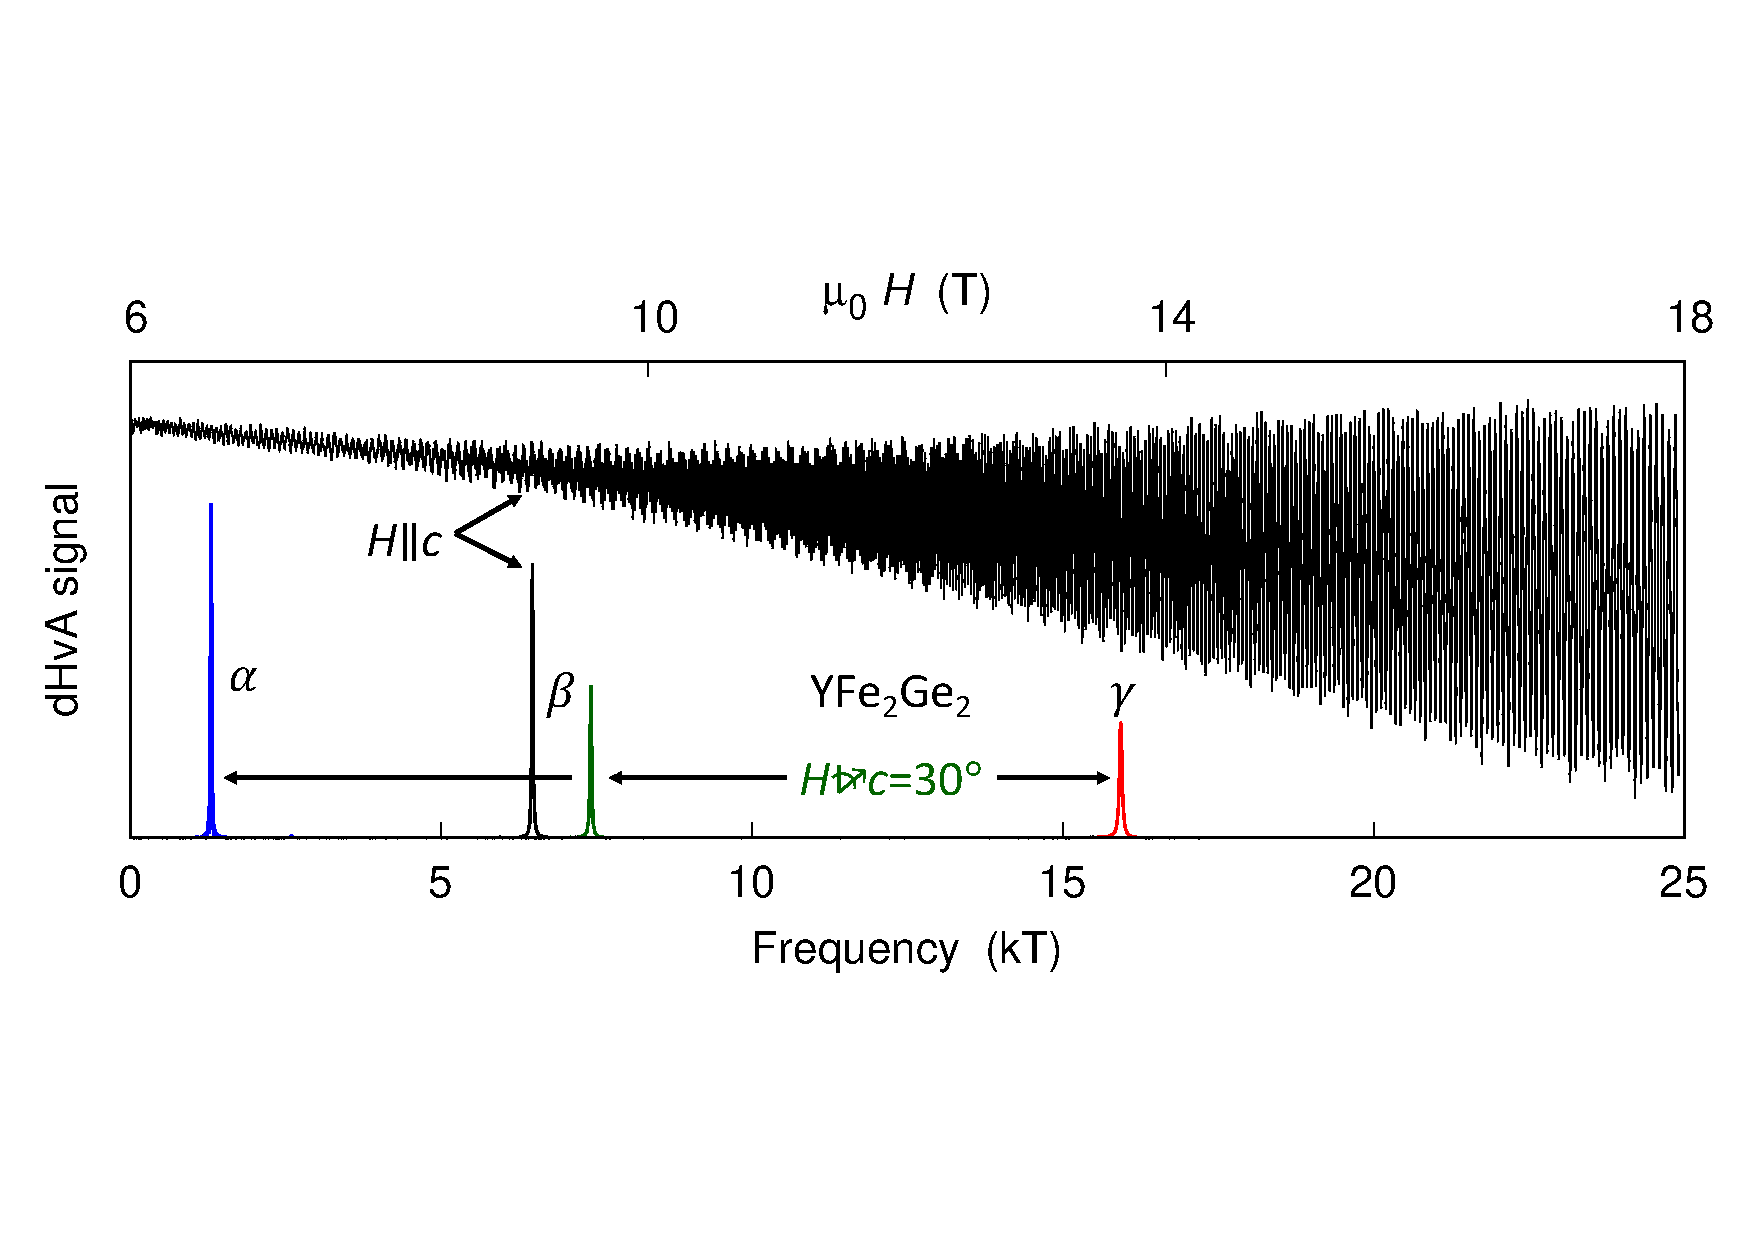
\includegraphics[width=\columnwidth]{Figures/YFGQOPlotFig}}
\centerline{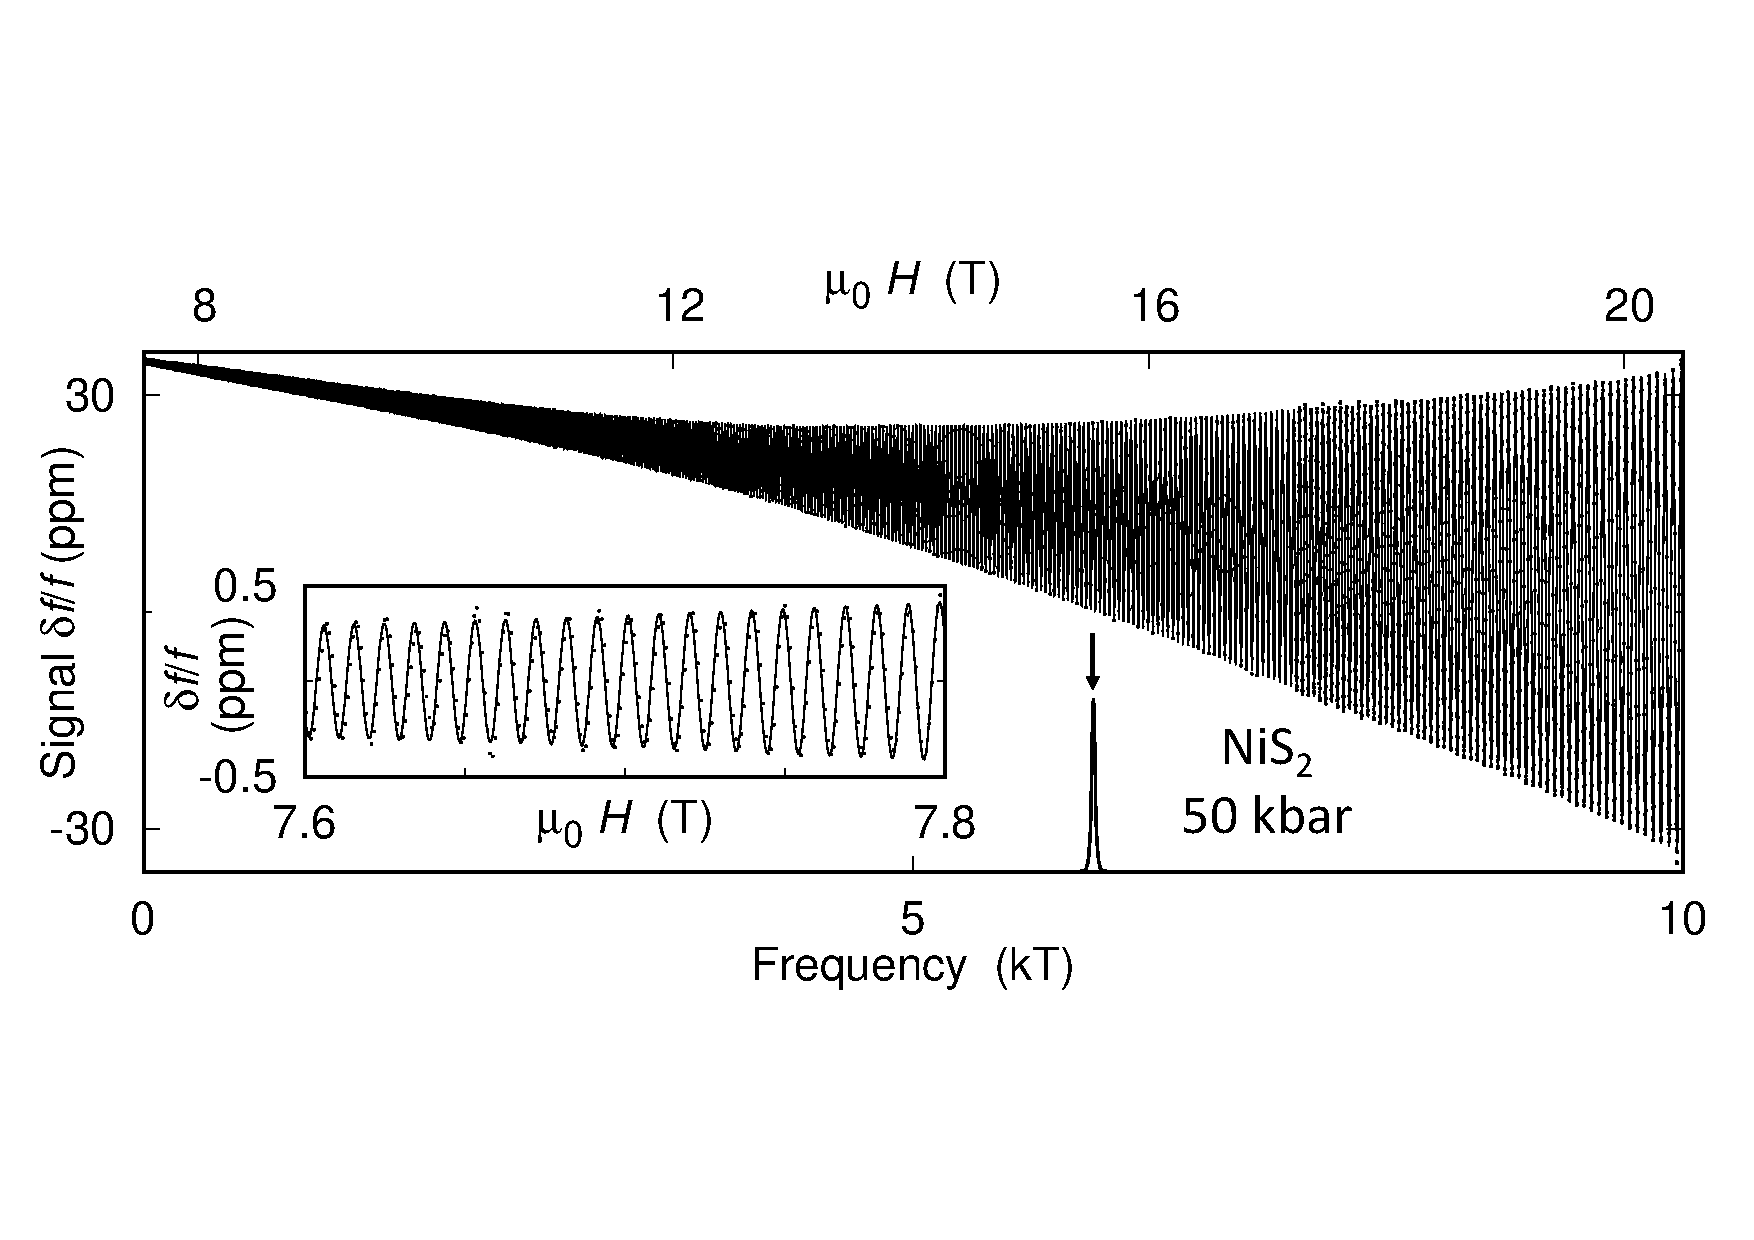
\includegraphics[width=\columnwidth]{Figures/NiS2QOPlotFig}}
 %\centerline{\includegraphics[width=0.75\columnwidth]{\Figures/Pressure/HighPQuantOsc/Ca2RuO4.pdf}}
\caption{{\bf Recent highlights:} The table lists selected
  publications in relevant areas. The figures show quantum oscillations signals recorded in the unconventional superconductor YFe$_2$Ge$_2$ (upper panel) \protect\citesel{baglo21} and in the correlated metallic state on the  threshold of Mott localisation in high pressure NiS$_2$ (lower panel) \protect\citesel{friedemann16,semeniuk22},
%  In both cases, the signal can be resolved down to  
%magnetic fields less than $8~\text{T}$
resolving key aspects of the electronic structure and demonstrating the high quality of in-house-grown crystals. }%The oscillation  frequencies give the extremal cross-sectional area of  the Fermi surface. 
%  The effective carrier mass, renormalised by interactions, can be derived from the temperature dependence of the oscillation amplitude. 
%  The high pressure data was obtained by tracking the  resonance frequency of an $LC$ oscillator, with the resonance coil  inside the sample volume of an anvil pressure cell \protect\citesel{semeniuk22}.}
\label{fig:Highlights}
\end{figure} 



% Moreover, the work will benefit from c
\subsection*{Key project partners} 
%{\em Geetha Balakrishnan}, Professor at the University of Warwick
% specialises in the growth of single crystals of superconductors and related magnetic materials. She will provide guidance and support on aspects of materials preparation for some of the systems, for example the rare earth hexa- and dodecaborides and skutterudites (objectives 1,3,4-7).

%{\em Alix McCollam}, Professor at Radeboud University and staff scientist at HFML Nijmegen ... \\
\paragraph{Antony Carrington, Sven Friedemann,} University of Bristol, will carry out penetration depth measurements using the tunnel-diode oscillator technique at ambient and elevated pressure and pursue transport and Raman measurements to ultra-high pressures.%electrical transport, neutron and x-ray studies on Cambridge-grown cuprate crystals. 

\paragraph{Devashibhai Adroja,} Rutherford Appleton Laboratory, will lead on muon spin rotation and neutron scattering studies of superconducting and magnetic states as well as magnetic excitations.

%\paragraph{Ingo Loa,} CSEC Edinburgh, will collaborate on high pressure structure determination using synchrotron x-ray sources.
%\paragraph {Juri Grin, Andrew Mackenzie, Manuel Brando,} MPI for Chemical Physics of Solids (Dresden/Germany), will analyse crystal quality by x-ray crystallography, SEM, TEM and other microscopic probes and carry out low temperature thermodynamic and dilatometric measurements.

\paragraph{Andrey Chubukov,} University of Minnesota, will contribute wide-ranging expertise in numerical
and analytic studies of quantum materials and help with interpreting experimental results. 


%{\em Monika Gam{z}a}, Lecturer at the University of Central
%Lancashire with long-standing expertise in crystal growth and crystallography, will carry out detailed characterisation by single crystal x-ray diffraction.
% . MG will bring expertise in careful characterisation measuresurements of single crystal samples, in particular using magnetisation \citesel{svanidze_itinerant_2015} and x-rays \citesel{gamza_electronic_2014}. Sample characterisation is especially important for studies in systems near phase transitions, as inhomogeneities can mask trends in tuning studies (objectives 1,3,4-7).


 




\subsection*{Research environment and prior work}
\noindent
The programme benefits from substantial prior work %on advanced measurement and cooling techniques 
(\autoref{fig:Highlights}) and from sustained investment
in modern research equipment, which includes a newly upgraded 20.4~T/dilution refrigerator high field
facility, a 15~T/300~mK cryomagnet, and a
7~T/100~mK cryogen-free demagnetisation cryostat.  Experiments demanding still higher
magnetic fields will be taken to international facilities, where we
have successfully bid for magnet time in the recent past (nine weeks since
2014). Two more weeks of magnet time at HFML Nijmegen have already been granted for work on this project. % For thermopower and
% thermal conductivity below 1K, we would mainly employ our 7~T/100~mK
% cryogen-free demagnetisation cryostat, and our 300mK Helium-3
% immersion probe.
A 9~T PPMS and a 7~T SQUID
magnetometer, both equipped with Helium-3 inserts, are available for sample
characterisation and rapid turnover measurements. %  A further
% 1~T/50~mK demagnetisation cyrostat is available for work at low
% magnetic fields. 
%  A 9T PPMS with Helium-3 insert and a 7T SQUID magnetometer
% with Helium-3 insert are available for sample characterisation and for
% quick high pressure measurements. A further 1T/50mK demagnetisation
% cyrostat is available for preliminary measurements. 
Crystal growth facilities include %UHV-compatible radio-frequency induction furnaces,
two arc furnaces and a mirror furnace as well as numerous box and tube
furnaces for flux and vapour transport growth. High-quality crystals of key materials in recent studies,
such as NiS$_2$ and YFe$_2$Ge$_2$, were produced in our group
(\autoref{fig:Highlights}).  
%Most of these facilities have been
%acquired % or upgraded
%over the last decade, demonstrating the commitment of the Cavendish
%Laboratory. % to this area of research.
Advanced electron-microscopy and x-ray characterisation
equipment as well as focused ion beam facilities are available within
the Cavendish, and we can access additional growth and
characterisation facilities at the new Henry Royce Institute for
Materials in Cambridge.



% Recent achievements (Fig.~\ref{Highlights}) include
% (i) discoveries made by tuning correlated systems near quantum phase
% transitions, (ii) high precision quantum oscillation, transport  (Fig.~\ref{ThermalCond}) or
% thermodynamic measurements at low temperature, in high magnetic
% field, and under applied pressure, 
% (iii) development of new techniques such as high pressure microcoil
% de Haas-van Alphen, NMR or
% tunnel diode measurements, high pressure
% SQUID magnetometry, and patterned
% anvil cells. 
% Members of the QM group have a proven track record of developing
% bespoke, precision instrumentation for the most demanding cryogenic
% measurements. Notable successes include the design and construction of
% diamond anvil and piston cylinder cells using micro pickup coils for
% quantum oscillation measurements under pressure \citesel{goh08},
% and the construction of a thermal transport stage for high resolution
% measurements at T~$<$~4~K \citesel{smith08}.
% Moreover, materials growth work carried out over the past year as part of an EPSRC
% Impact Acceleration Grant has established the procedures for producing large pills
% of metallic magnetocalorics, a central ingredient for the envisaged compact, robust and efficient
% sub-Kelvin adiabatic demagnetisation refrigerators.
%  through the manufacture of large scale
% samples of metallic magnetocalorics.
% Through this programme we have
% developed an understanding of the growth of samples of metallic
% refrigerants, which will inform the materials preparation aspects of
% our research plan.

\vspace{-1em}

\bibliographystylesel{apsrevFMG}

\bibliographysel{References}

% \end{document}

%%% Local Variables:
%%% mode: latex
%%% TeX-master: "Case"
%%% End:

%\clearpage

%\fontsize{10.87pt}{12.1pt}\selectfont
\setlength{\columnsep}{2em}
% !TEX root = UCase.tex
% \vskip -1em
\onecolumngrid
% \begin{center}
% %{\bf{\em \large Unconventional superconductivity in the layered intermetallic YFe$_2$Ge$_2$}}\\
% %{\bf{\em \large Unconventional superconducting and normal states in transition metal compounds -- a new generation of ultra-pure crystals}}\\
% %{\bf{\em \large Origins of mass renormalisation and unconventional superconductivity in transition metal compounds}}
% %{\bf {\em \large Superconducting and normal states in quantum materials  \\}}
% %Unconventional superconducting and normal states \\ in transition metal compounds\\}}
% %\vspace{2em}
% { Part 2: Case for support}
% \vspace{-1em}
% \end{center}

\begin{mdframed}[hidealllines=true,backgroundcolor=blue!5,innerleftmargin=5pt,innerrightmargin=5pt,innertopmargin=5pt,innerbottommargin=5pt]
\noindent
Uranium-based unconventional superconductors are surprisingly abundant and continue to defy a comprehensive understanding. Foremost among these is the new superconductor UTe$_2$,  which displays at least three distinct superconducting states and in which superconductivity can survive up to fields exceeding \SI{60}{\tesla}, indicating triplet pairing. With ultra-clean crystals of UTe$_2$ now available, this project combines wide-ranging experimental, computational and theoretical studies into the origins of superconductivity and the associated anomalous normal states in UTe$_2$ and related uranium-based quantum materials. % that represent a broad spectrum of electronic and vibrational energy scales.
%that include (i) the new iron-based superconductor YFe$_2$Ge$_2$, now available at unprecedented purity levels that exceed the best crystals grown outside Cambridge by at least an order of magnitude, (ii) the quantum critical heavy fermion superconductor CeNi$_2$Ge$_2$, for the first time now available as high purity single crystals suitable for quantum oscillation studies, (iii) the newly discovered unconventional high pressure superconductor CeSb$_2$, which shows ultra-strong electronic correlations and an unusually high critical field that far exceeds the paramagnetic limit, (iv) quasi-periodic host-guest structures such as high pressure Sb-II and Ba-IV, which feature low-lying sliding modes that facilitate strong-coupling superconductivity. 
%Our findings will refine the criteria guiding the search for new superconductors, increasingly  targeted for  practical applications.
\end{mdframed}
% \vspace{1em}
%   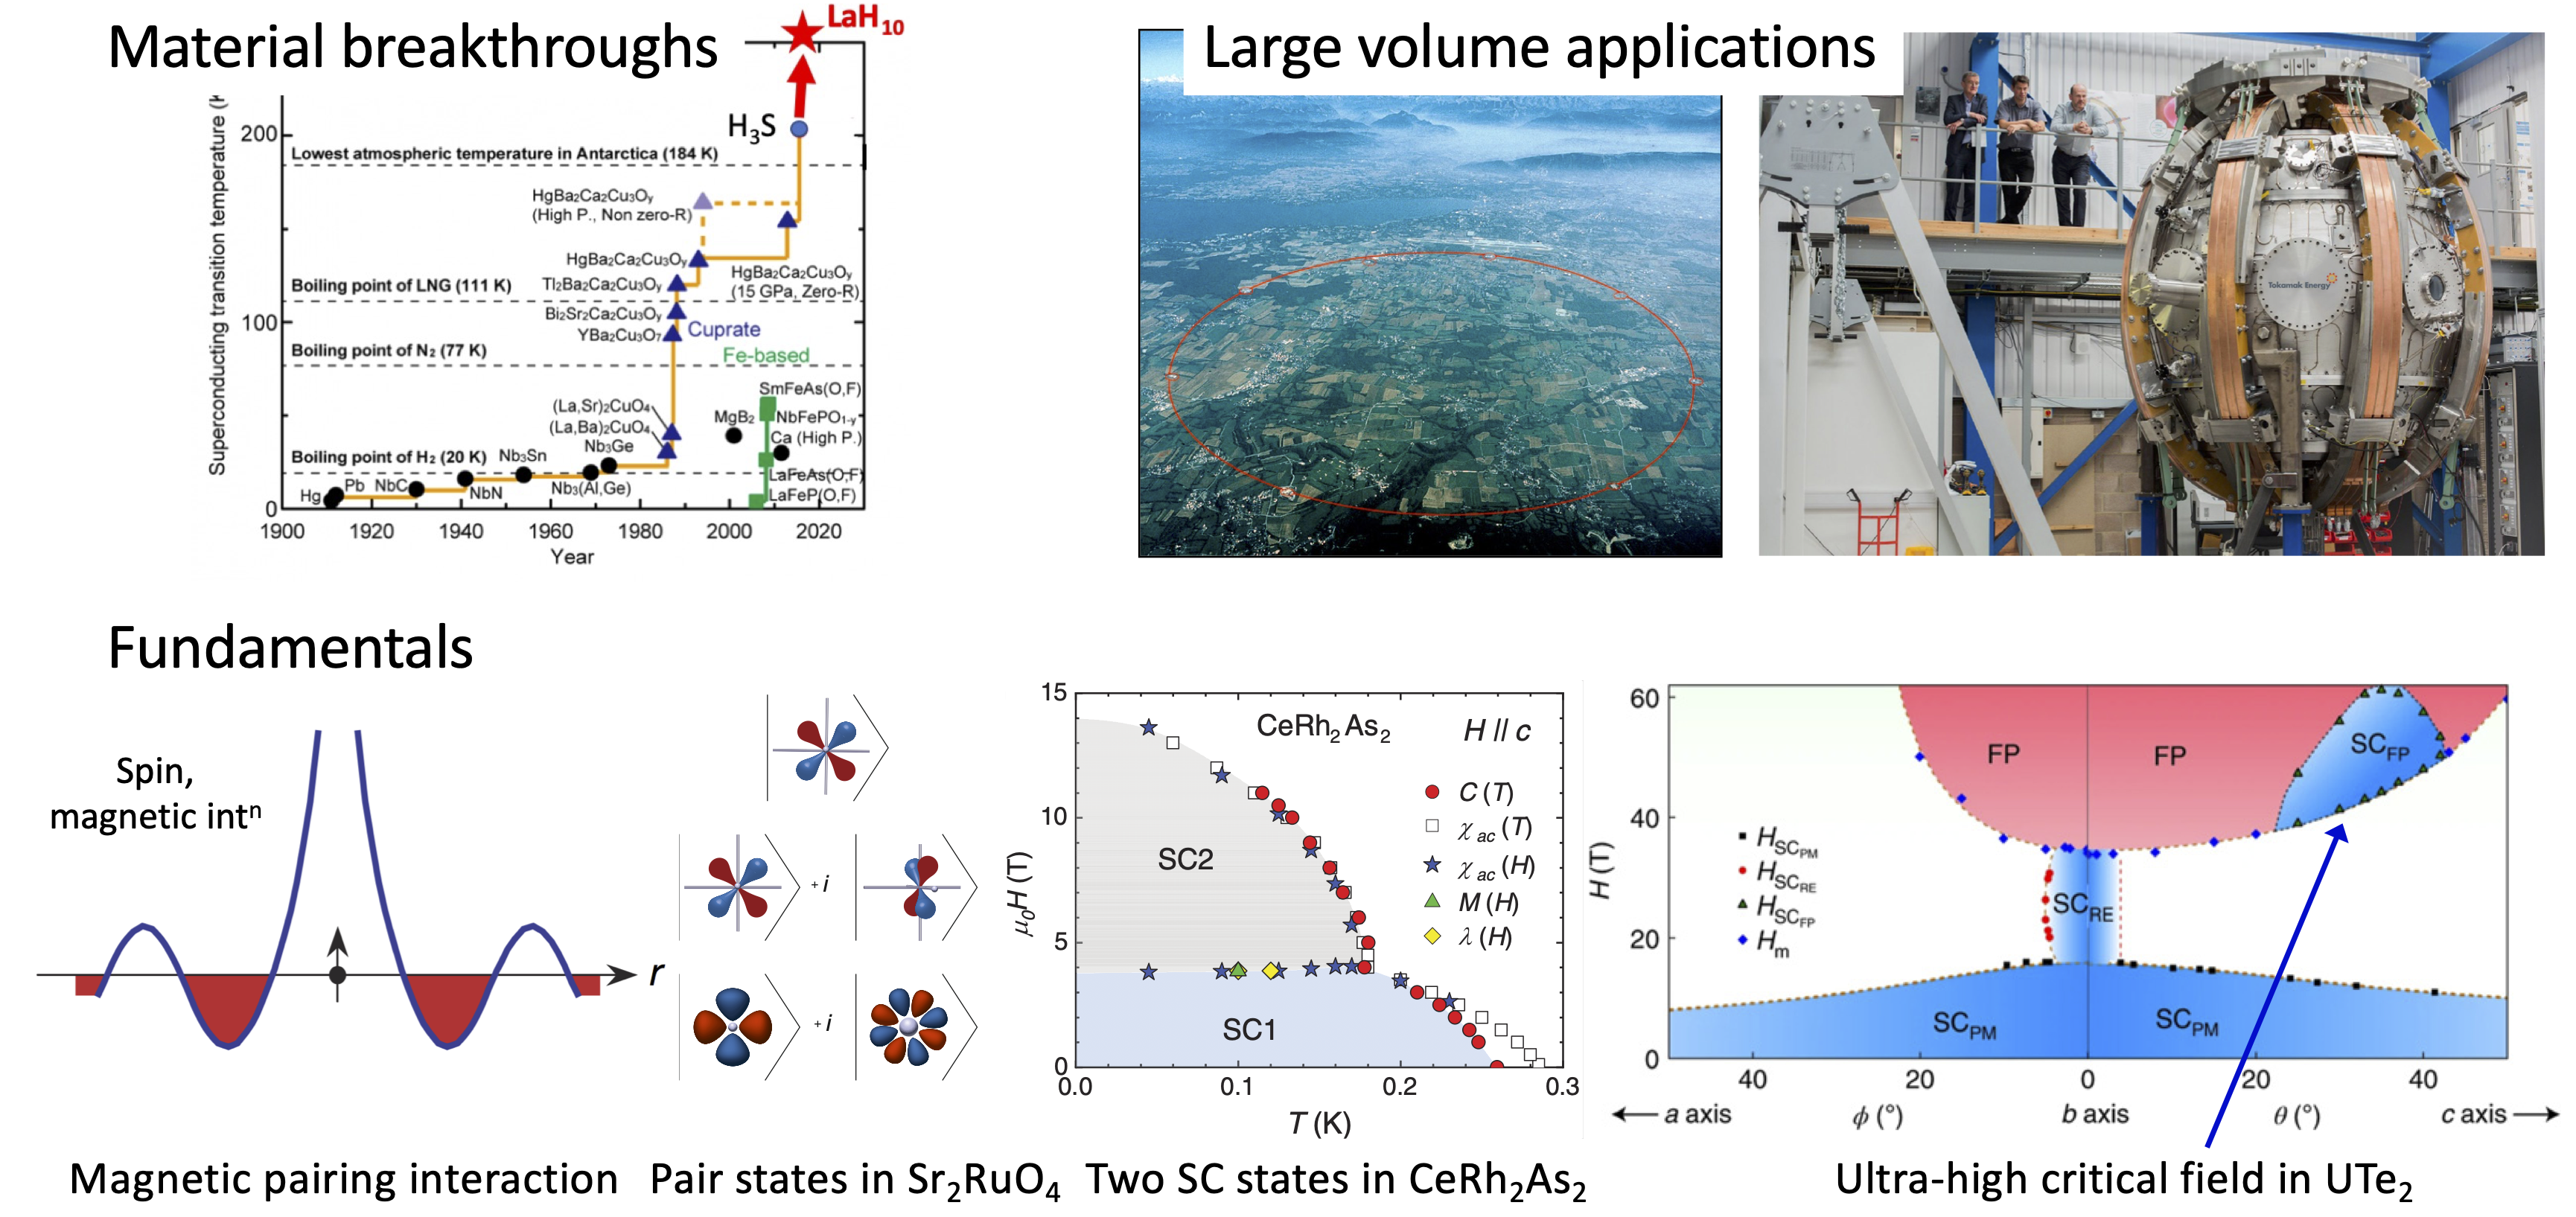
\includegraphics[width=\columnwidth]{Figures/SuperconResurgent2}
  
\twocolumngrid

%Note: include references to potential referees:  Sebastian, Balakrishnan, \\

\subsection*{Superconductivity resurgent}
\noindent
Superconductivity research is ramping up globally, driven by (i) the recognition that superconductors facilitate large-volume applications for instance in fusion research, accelerators, MRI scanners, generators and motors, and power distribution, as well as device applications in computing and sensing; (ii) exciting breakthroughs in fundamental research across different material systems ranging from the cuprates and Fe-based high temperature superconductors to organics, twisted bilayer graphene and f-electron systems; (iii) materials breakthroughs, including the ability to induce near-room temperature superconductivity %under extreme pressure 
in supercompressed superhydrides \cite{drozdov19,somayazulu19}, the discovery of \SI{80}{\kelvin} superconductivity in a pressurised, novel nickelate \cite{sun23}, and the discovery of multiple field resilient superconducting states in CeRh$_2$As$_2$ \cite{khim21} and UTe$_2$ \cite{aoki19,ran19}. 


% One of the most exciting recent developments in condensed matter research has been the
% demonstration of \myul{superconductivity in superhydrides} near room temperature but at very high pressure
% \cite{snider20,drozdov19,somayazulu19}. 
% The compressed superhydrides demonstrate the power of engineering a phonon-mediated superconducting pairing mechanism towards optimal outcomes. Further gains are possible by widening the scope towards 
%In compressed superhydrides such as LaH\textsubscript{10}, superconductivity is mediated by dynamic deformations of
%the crystal lattice which, because of the light mass of the hydrogen
%atoms and the high spring constants caused by strong compression, reach
%to very high frequencies. This approach could produce
%high temperature superconductivity at ambient pressure, if -- like diamond -- a metastable high pressure structure could be brought back to ambient conditions. %This is not the case for LaH$_{10}$. 

In conventional superconductors, the pairing interaction is communicated by lattice vibrations. Fundamental and applied superconductivity research are increasingly examining \myul{unconventional superconductors}, which instead harness the {strong electronic interactions} that are also responsible for magnetism and that are
known in some cases to reach coupling strengths equivalent to several
thousand Kelvin \cite{monthoux07,norman11}. Like rare minerals that occur in seams, these superconductors are thinly spread across the space of all accessible materials but richly concentrated within those families on which most current research is focused, which include, for example, various copper oxide, iron or cerium compounds. 

%Unconventional superconductivity in cuprates, for instance, has already produced transition temperatures $T_c$ approaching $160~\text{K}$. To optimise the effects of direct
% electronic interactions further requires a better understanding of the underlying and often competing
% mechanisms in these complex materials. 
%Medium-term commercial impact will arise from new materials identified as a consequence of our research. Our experimental results will help refine numerical models that will guide the search for new superconductors with high volume applications, including those mentioned in the introduction above. 

%Only a few material families are so far known to exhibit superconductivity that is not mediated by lattice deformations, or phonons, alone \cite{monthoux07,norman11}. 

\paragraph{Uranium-based superconductors} make up a large fraction of the overall still limited number of unconventional superconductors (Table). This material family is highly diverse in terms of crystal and electronic structure. %Superconductivity in U compounds is often found near the threshold of ferromagnetism, but many U superconductors are antiferromagnetic or appear far from the threshold of magnetism. 
Studying and learning from these U-based superconductors can accelerate the wider search for unconventional superconductors with desirable properties, but the bewildering diversity and complexity of phenomena and materials challenges in this class of materials renders a detailed and comprehensive understanding at best time-consuming and difficult. 

\begin{figure}
  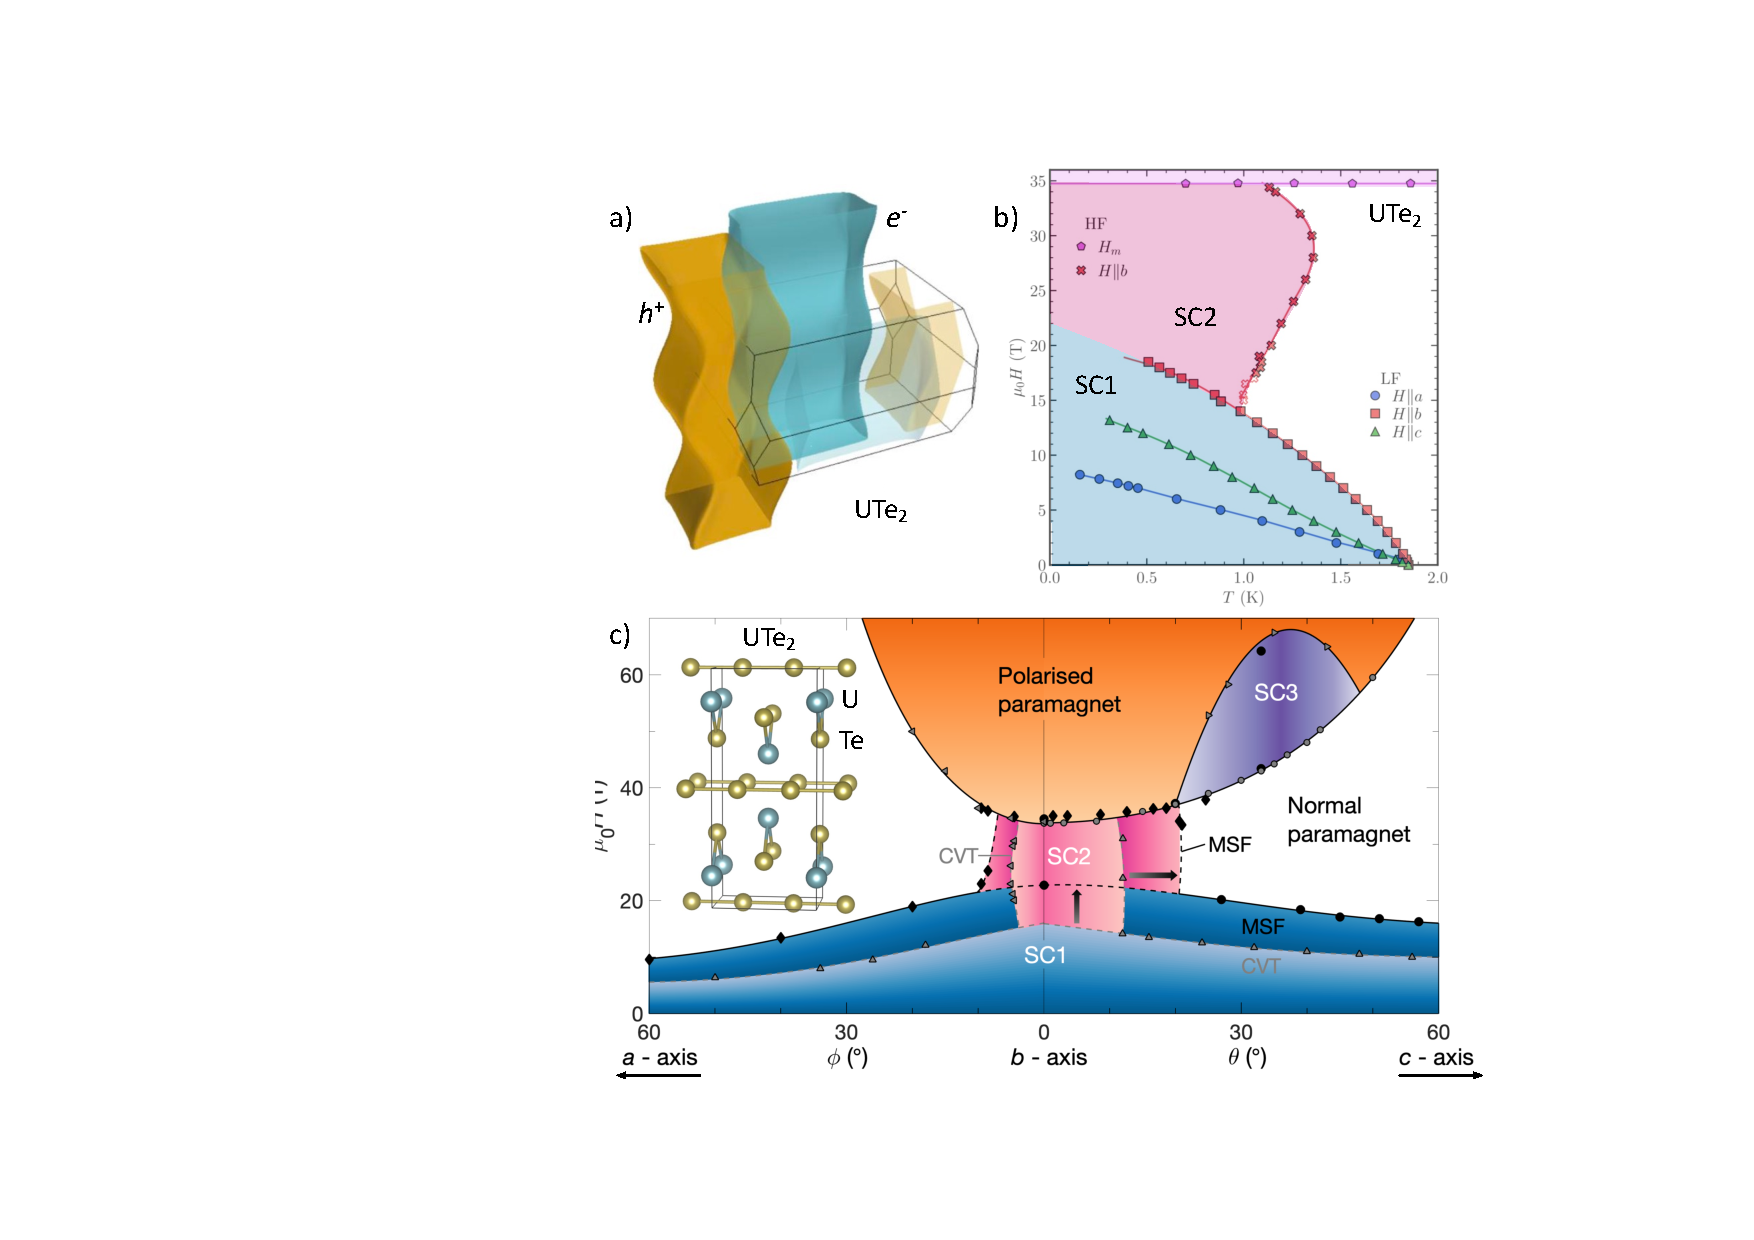
\includegraphics[width=\columnwidth]{Figures/UTe2Overview.pdf}
  \caption{{\bf Key properties of UTe$_2$.} (a) Crystal structure and Fermi surface geometry deduced from quantum oscillation measurements, showing compensated electron and hole pockets of constant cross-section that undulate slightly along the $c$-axis. (b) Temperature dependence of the superconducting upper critical field $B_{c2}$ along the $b$-axis, showing transition between two superconducting states, SC1 and SC2. (c) Angle dependence of the low temperature $B_{c2}$, showing the resilience of SC2 to applied fields reaching up to a metamagnetic transition at $\simeq \SI{35}{\tesla}$ and a third superconducting state SC3 that reaches to far higher field values, still. Our improved 'MSF' crystals reach higher critical fields in the SC1 state (dark blue) and superconductivity extends over a wider angle range in the SC2 state (pink) than previous 'CVT' generations of samples.}
  \label{fig:UTe2}
\end{figure}

\paragraph{The new superconductor UTe$_2$} presents a clean model system, in which numerous layers of complexity are stripped away to reveal underlying principles that can be studied and understood with current methods. After initial studies were hampered by poor crystal quality, new growth methods pioneered by our project partners now produce pristine single crystals with superior quality and electronic mean free path. In these crystals, direct measurements of the electronic structure near the Fermi energy are possible, and have revealed a surprisingly simple Fermi surface geometry, which consists of just two cylindrical, slightly corrugated pockets (\autoref{fig:UTe2}).
%and our group has played a leading role in discovering several such examples \cite{mathur98,saxena00,grosche00,zou14}.
% We urgently need to find new unconventional superconductors: 
% %they present proving grounds for advanced computational techniques, generate fresh impulses that advance our understanding of superconducting quantum materials in general and thereby prepare the ground for the next discovery,  helping us formulate guiding principles -- heuristic filters needed to select promising candidate systems. 
% not only are they scientifically interesting -- with every case  studied, the guiding principles for finding new superconducting material families can be refined.
% An example of such a guiding principle is illustrated in \autoref{fig:Guiding}, namely to home in on the threshold of magnetic order. There, at a so-called  \myul{quantum phase transition}, magnetic excitations reach to low energies. They mediate a long-ranged interaction which can stabilise superconductivity with an unconventional order parameter structure %(e.g. $s_\pm$, $p$- or $d$-wave)  
% \cite{monthoux07}. Such non-phononic pairing interactions are strongly tuneable. This causes superconducting domes 
% %as in Fig.~{\ref{fig:Guiding} 
% which in some cases are surprisingly narrow, explaining why this type of superconductivity is often found not by random searches but by scanning phase diagrams systematically near the border of magnetism. % -- for which high pressure studies are well suited.


\begin{figure*}
  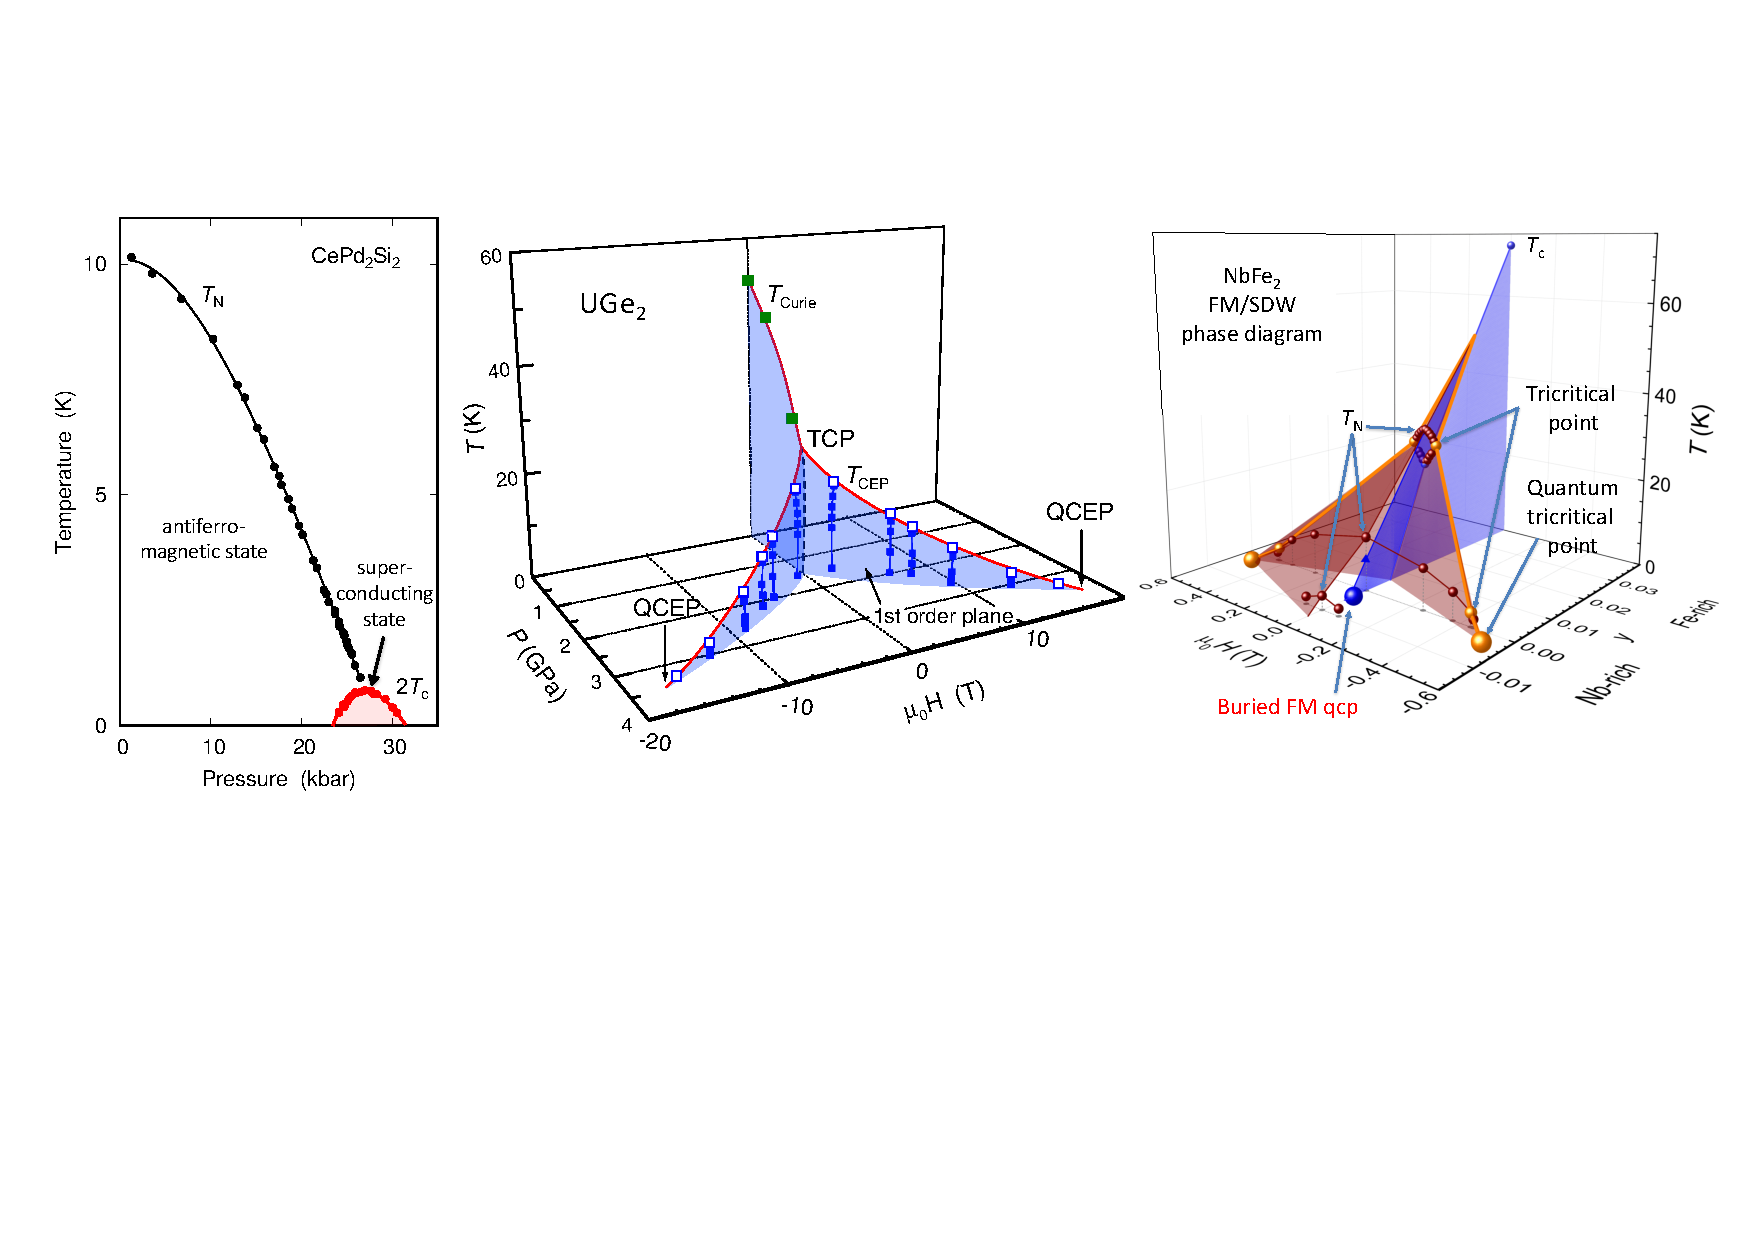
\includegraphics[width=1.9\columnwidth]{Figures/PhaseDias.pdf}
  \caption{{\bf Template phase diagrams guiding materials exploration:}  (a) High pressure phase diagram of CePd$_2$Si$_2$, showing a superconducting region attached to the 
  threshold of antiferromagnetism \protect\citesel{mathur98}. Considering the added effect of magnetic field adds a third dimension:
  in UGe$_2$ (b), 
  superconductivity appears within a ferromagnetic region, which itself branches into two metamagnetic sheets \protect\cite{kotegawa11}. In PrPtAl or NbFe$_2$ \protect\citesel{friedemann18} (c), by contrast, ferromagnetism is replaced by an antiferromagnetic or spin-density wave region.
  %With hindsight, the  observation that iron-based superconductivity often peaks near the disappearance of magnetic order, whether achieved
  %by doping or pressure, resonates with the earlier realisation that low-\emph{T}\textsubscript{c} Ce-based
  %superconductors are frequently found on the threshold of magnetism. 
}
  \label{fig:Guiding}
  
\end{figure*}
  
  




%The discovery of new unconventional superconductors often appears to happen randomly, although with hindsight some may have been anticipated. 
%The searches that led to these discoveries were guided by theoretical principles, most prominently the exploration of quantum phase transitions. The success of these searches suggests that the time may be right for a systematic programme of exploration (\autoref{Prospecting}),


%Importantly, however, %things are not usually as clean-cut as suggested by \autoref{fig:Guiding}, and 



\begin{figure}[t]
%  \centerline{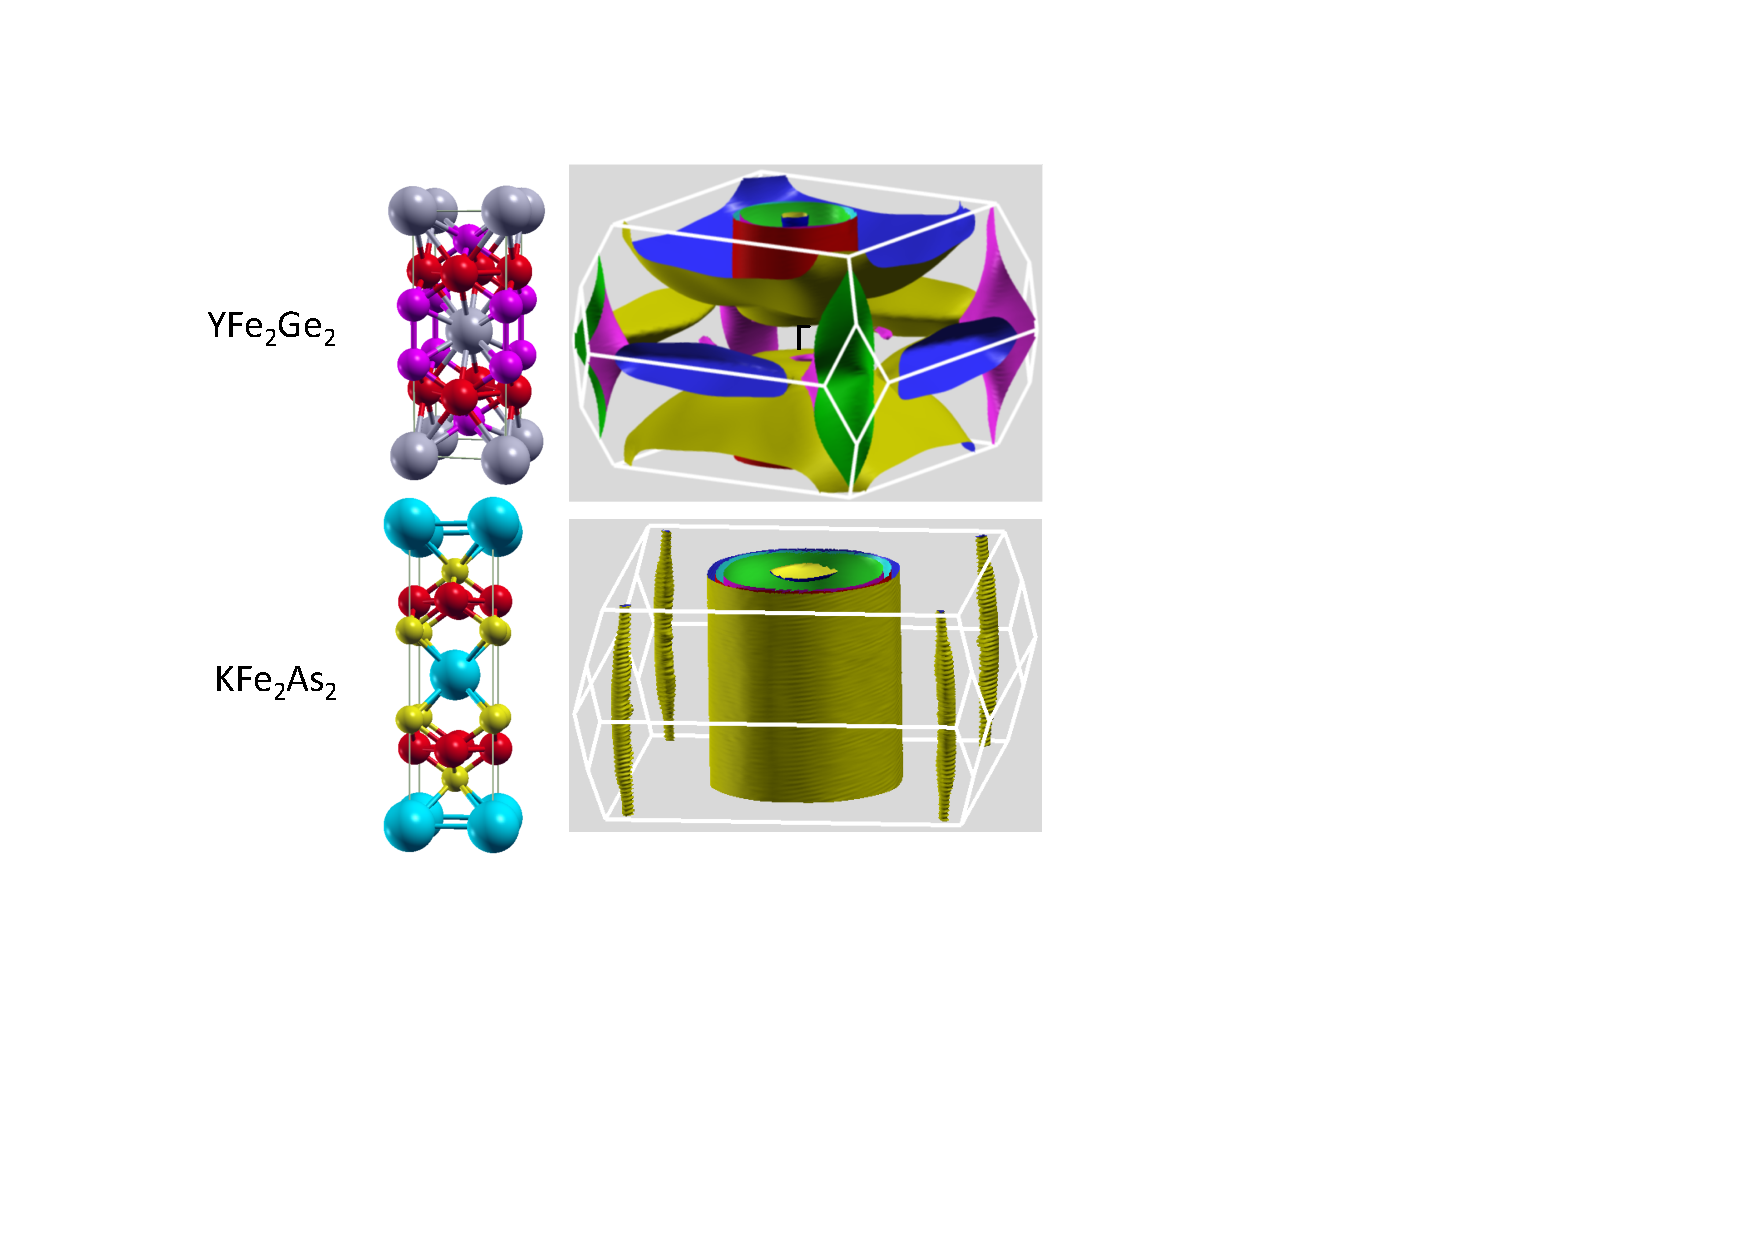
\includegraphics[width=0.95\columnwidth]{Figures/CompareKFA-YFG3b}}
\centerline{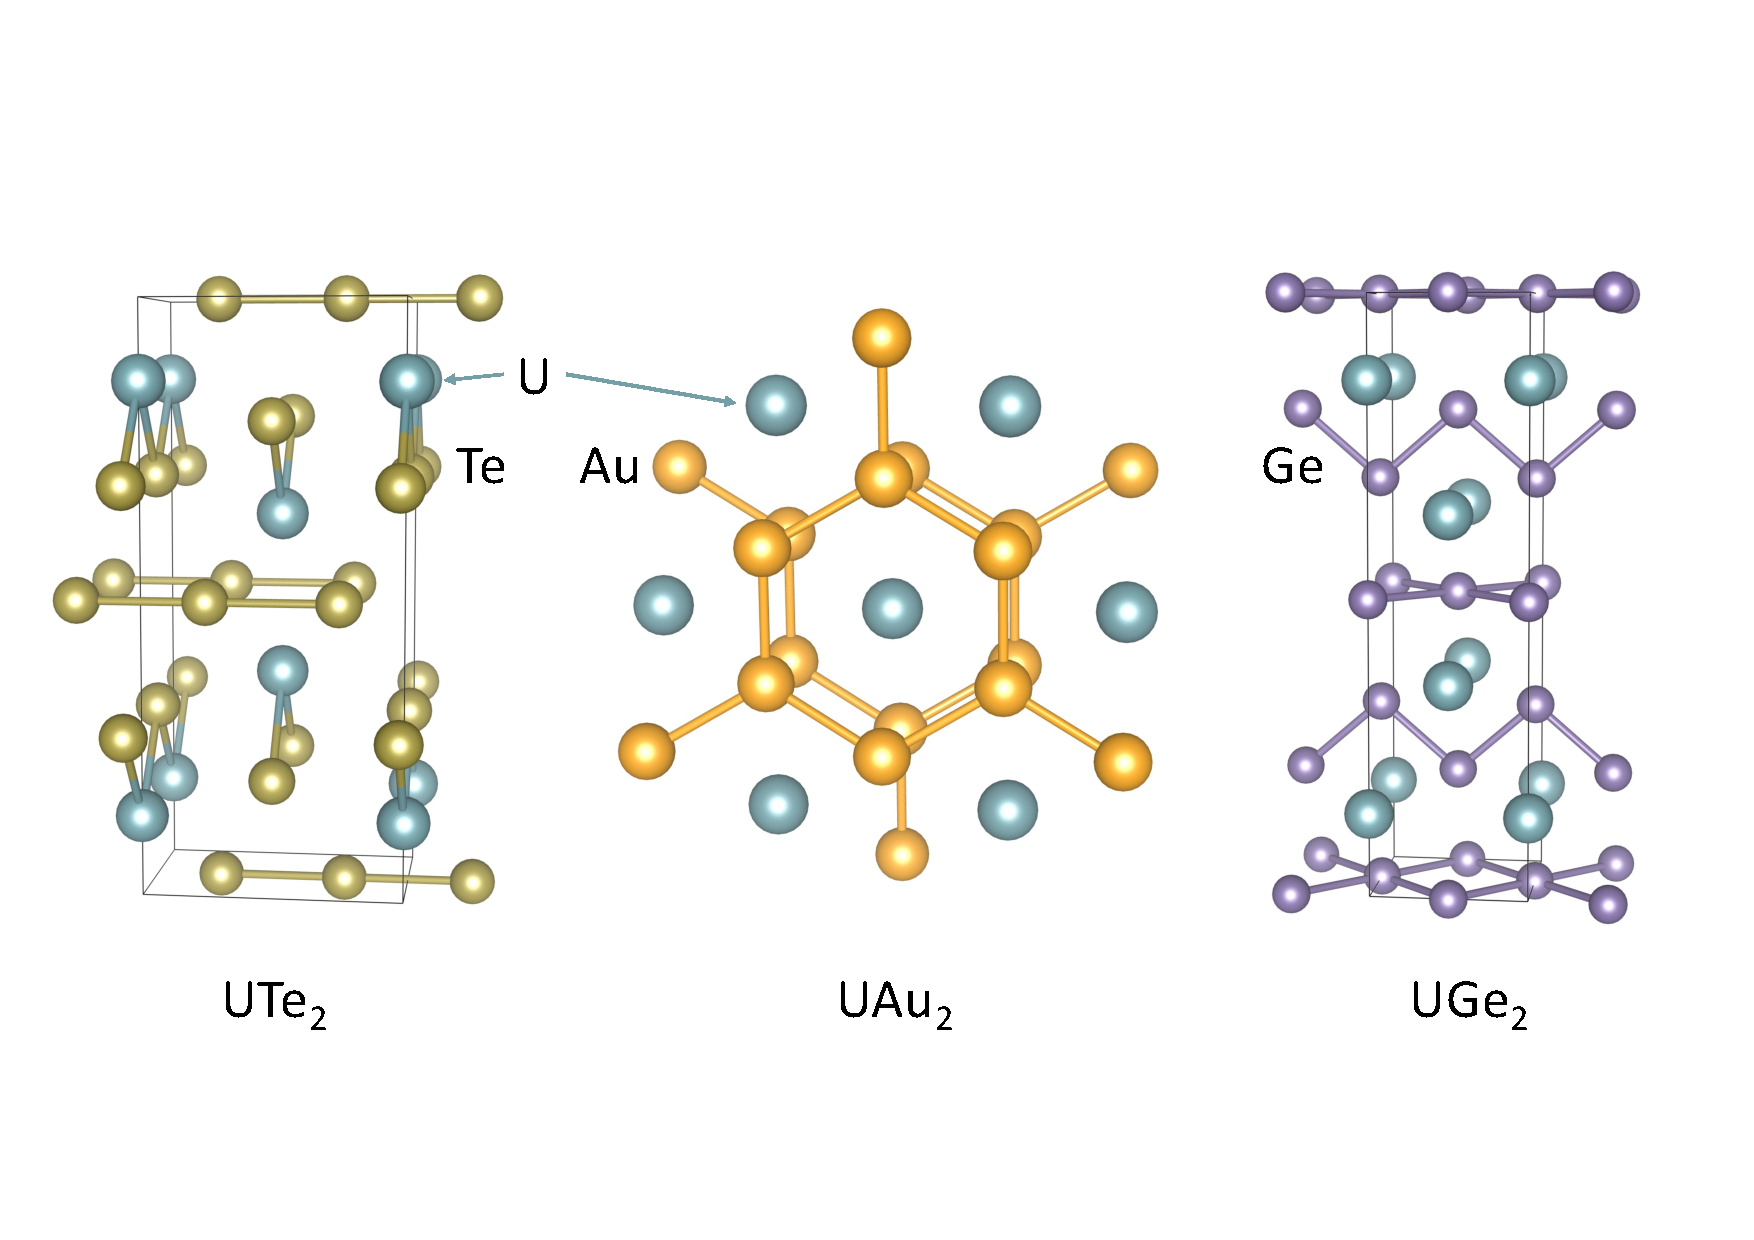
\includegraphics[width=\columnwidth]{Figures/Structures.pdf}}

   \caption{{\bf Material families} identified for the first stage of this project. As the programme unfolds, the investigation will widen first to other U-based superconductors (see table) and eventually to $d$-metal compounds with strong Hund's coupling and hence underlying similarity to the headline materials. }
   
    \label{fig:Materials}
\end{figure}


\subsection*{Research questions}
\noindent
Our project will address the following \myul{key research questions} of wider relevance in superconducting quantum materials:

% These four material families span a broad range of electronic energy scales, from the low Kelvin regime in high pressure CeSb$_2$ to thousands of Kelvin in Bi, Sb and Ba, with YFe$_2$Ge$_2$ %($\sim \SI{400}{\kelvin}$) 
% and CeNi$_2$Ge$_2$  %($\sim \SI{100}{\kelvin}$) 
% connecting the two extremes. Nevertheless, they share striking similarities, such as tunability by pressure or composition and proximity to magnetic or structural instabilities. 
% Above their superconducting transitions, they all exhibit anomalous `normal' states with a sub-quadratic temperature dependence of the electrical resistivity, signalling low-lying excitations. In Bi-III (\autoref{fig:Materials}d), this non-Fermi liquid form of the resistivity may be attributed to low-lying sliding \ul{phonon} modes, which are a built-in consequence of its quasiperiodic structure. %This illustrates the central role of soft modes for causing anomalous electronic transport properties and also for understanding strong-coupling superconductivity. 
% By contrast, \ul{magnetic} excitations that become long-lived and long-range near the threshold of magnetism likely play the dominant role in the other three material families. 

%Exploiting these contrasts and similarities, 


\paragraph {a) Superconducting state:} what is the symmetry of the superconducting order parameter? What causes high critical fields, in particular if they far exceed the paramagnetic limit? %as in high-pressure CeSb$_2$? 
What is the origin of residual $C/T$ in the low $T$ limit in many samples of unconventional superconductors such as UTe$_2$, and can this be quantitatively attributed to impurity bound states? 
Can we explain not only why some materials superconduct but also why other, very similar materials do not? What factors determine the variation of $T_c$ within the same material family? 

%Superconducting properties will be investigated in multi-probe studies with a wide range of collaborating groups (see below), in some cases in combination with applied pressure.

\paragraph{b) Anomalous `normal' state:} % out of which the superconductivity emerges:
superconductivity arises out of a strongly correlated normal state. What is the origin of the high electronic heat capacity and enhanced quasiparticle mass in UTe$_2$ and other U-based heavy fermion compounds, which typically exceeds density functional theory (DFT) values by at least an order of magnitude? Although there will be parallels with 4{\em f}-electron systems such as the Ce- and Yb-based heavy fermion compounds, many U-based superconductors have two or three {\emph f}-electrons on each U site. This introduces strong local correlations via \myul{Hund's coupling}, which may produce significant baseline mass renormalisation, as demonstrated, for instance, in our work in YFe$_2$Ge$_2$ \cite{baglo22}. 

%A breakdown of the standard model of condensed matter physics, Fermi liquid theory, can be signalled by a sub-quadratic temperature dependence of the electrical resistivity $\rho(T)$ at low temperature. 
%Such anomalous forms of the resistivity have been observed in many materials, including cuprates, iron based superconductors such as YFe$_2$Ge$_2$ and other transition metal compounds, heavy fermion compounds, but also in 
%Similar phenomena can also be attributed to low-lying phonon modes, for instance 
%the high-pressure structure of Bi and the quasi-skutterudite Ca$_3$Ir$_4$Sn$_{13}$ near a structural qcp \citesel{klintberg12}. 
%Understanding this wide-spread phenomenon  (e.g. \autoref{fig:Materials}, but also other heavy fermion and transition metal compounds such as the cuprates), which often coincides with unconventional or strong-coupling superconductivity, is a fundamental challenge in condensed matter physics. 
%Are signatures of Fermi liquid breakdown confined to the immediate vicinity of quantum critical points?
% or can they extend over regions in parameter space? 
%Can they be understood quantitatively in terms of observable low-energy excitations, or soft modes -- charge, orbital, nematic, magnetic or vibrational? How do they relate to \myul{Planckian dissipation} (e.g. \cite{bruin13,hartnoll15}) as a universal ceiling on scattering rate? 
%We will investigate signatures of Fermi liquid breakdown in transport, magnetic or thermodynamic properties or even in quantum oscillation measurements and track them with applied field, composition and pressure. 

\paragraph{c) Nature and tunability of effective interaction:} superconducting and normal state properties are controlled by the effective interaction between charge carriers, or quasiparticles. In contrast to the bare Coulomb interaction, the effective interaction can be dynamic, it can couple to spin, and it can be tuned by varying underlying material parameters. In many currently known unconventional superconductors, the interaction is predominantly magnetic \cite{monthoux07}, but different mechanisms are possible. These might involve density, valence, quadrupolar or orbital degrees of freedom, individually or in combination. How does the form of the effective interaction connect to microscopic models such as the Hubbard model for correlated metals near Mott localisation, the Kondo lattice model for 4$f$-electron heavy fermion superconductors, or the Hund's metal in some of the Fe-based superconductors \cite{georges13}? 
%In the latter,  the electrons in the far more extended Fe $d$-states, which are forced into a high spin state, introduce strong local correlations that may be seen as analogous to Kondo lattice physics. Is this conceptual connection between rare-earth based heavy fermion compounds and the newer Fe-based superconductors helpful in understanding both material families?
%Can the Kondo energy be tuned to zero in special cases, as proposed in scenarios of orbitally selective Mott transitions or Kondo breakdown (e.g. \cite{si01,paul07}), and what are the consequences of ultra-low Kondo scales for superconducting and normal state properties? %What is the relationship between the underlying crystalline, electronic and magnetic structure and the form of the effective quasiparticle interaction? 
Can we understand and control the energy scales that enter these microscopic models,  and can we exploit their tunability to vary superconducting and normal state properties? 
%At a microscopic level, rare-earth based, so-called heavy fermion superconductors are often discussed in a Kondo-lattice model in terms of the interplay between electrons in extended $s$, $p$ and $d$-states, which form broad metallic energy bands, and more localised electrons in tightly confined $f$-states, which take on properties of local magnetic moments at high temperatures or high energies. 
%A crucial parameter in this picture is the Kondo energy scale, which sets an effective bandwidth in the low temperature limit.
%How can aspects of the effective interaction be varied, for instance by changing composition or pressure, to affect normal state properties, the superconducting transition temperature $T_c$ or critical fields?   

More ideas: \\
\begin{itemize}
  \item Most early hf superconductors were U-based. Maybe because it's actually wide-spread in U compounds? 

\item $C/T$ is intermediate between heavy d-metal compounds (e.g. KFe2As2, YFe2Ge2) and Ce-compounds

\item
Local vs. band, orbitally selective Mott transitions? What is the number of itinerant f electrons? 
Age-old problem of e.g. UPt3 QO

\item 
On-site correlations, Hund's metal 
How do we actually pick that up experimentally?

\item
Role of Spin-orbit coupling?

\item 
FM qcp -> 1st order or SDW or something else altogether (URu2Si2). 
Lessons from NbFe2, PrPtAl

\item 
What determines Bc2, and what can we learn from it? 
And are there ways to maximise Bc2?

\item 
Are there vortex state transitions?
Maybe lessons to be learned for applications

\item 
Multicomponent order parameters
How do we identify them? How are they manipulated? How can we find new materials that host them?

\item 
Fermi surface instabilities
Central e.g. to UGe2 story. Maybe happens more generally?!

\item Nature of hidden order states, as in URu$_2$Si$_2$

\end{itemize}

\subsection*{Selected materials}
\noindent
% Driven by this overarching objective, 
For these reasons, our project will initially investigate three material systems available as \myul{high-quality single crystals}, in which discoveries and enabling breakthroughs %in crystal growth and high pressure techniques 
have occurred as recently as last summer (\autoref{fig:Materials}):
%Recent discoveries and advances in crystal growth and high pressure techniques enable a broad study across four material systems, which 
%The chosen materials display common phenomena but access a wide range of electronic or vibrational energy scales  (\autoref{fig:Materials}):
%the new \uline{iron-based superconductors} YFe$_2$Ge$_2$ and LuFe$_2$Ge$_2$, the \uline{moderate heavy-fermion superconductors} CeNi$_2$Ge$_2$ and CePd$_2$Si$_2$, the \uline{ultra-heavy fermion superconductor} CeSb$_2$ and the \uline{quasiperiodic superconductors} high pressure  Bi, Sb and Ba.
%We will investigate four superconducting material systems  

\paragraph {a) UTe$_2$:} 
%including the new system YFe$_2$Ge$_2$ and its relative LuFe$_2$Ge$_2$, which straddle an antiferromagnetic quantum phase transition and exhibit  an unusually high heat capacity $C$ at low temperature $T$ ($C/T \simeq 100~\text{mJ/molK}^2$), consistent with our observation of carrier mass renormalisation among the highest recorded in transition metal compounds \citesel{baglo21}. 
% Whereas LuFe$_2$Ge$_2$ is antiferromagnetic below about $\SI{6}{\kelvin}$, its isoelectronic sister compound YFe$_2$Ge$_2$ is paramagnetic. 
using a new generation of ultra-clean crystals grown using the molten salt flux technique by project partners at Charles University, Prague, we were able to detect quantum oscillations with unprecedented clarity, enabling us to resolve the Fermi surface structure of UTe$_2$ \cite{eaton23}. These high quality crystals with residual resistivity ratio (RRR) of order 500 display a significantly enhanced $T_c$ compared to previous generations of samples. Because disorder is always relevant in unconventional superconductors, many initial findings in UTe$_2$, starting with the observation of residual Sommerfeld ratio $C/T$ within the superconducting state, need to be re-examined in these new crystals. We have already found that the superconducting critical fields are significantly enhanced, whereas the metamagnetic transition remains unchanged \cite{wu23}. With at least three distinct superconducting states reported in UTe$_2$ in a complex field/pressure/temperature phase diagram, these new, cleaner crystals offer the opportunity to clarify many of the open scientific questions surrounding this interesting but complex material.


% discovered superconductivity in YFe$_2$Ge$_2$ \citesel{zou14,chen16,chen19}, emerging out of an anomalous normal state with a %non-Fermi liquid 
% $T^{3/2}$ power-law dependence of the resistivity. 
% %The non-Fermi liquid $T^{3/2}$ form of the electrical resistivity, the pronounced effect of disorder scattering on superconductivity \cite{chen19} and theoretical studies \cite{singh14,subedi14} indicate that YFe$_2$Ge$_2$ is an unconventional superconductor. 
% More recently, we also found superconductivity in the newest generation of high purity crystals of LuFe$_2$Ge$_2$ (\autoref{fig:Materials}a). 
% These findings depended on our ability to produce ultra-high quality crystals of both materials, with purity levels in YFe$_2$Ge$_2$ exceeding those of the best samples grown outside Cambridge tenfold \citesel{chen20b}. %This new generation of crystals will enable wide-ranging multi-probe studies in both materials as well as non-superconducting reference compounds, which will be outlined below.


\paragraph{b) UAu$_2$:}
\highlight{Text about UAu$_2$} 
% compounds such as CeNi$_2$Ge$_2$ and its relative CePd$_2$Si$_2$, which likewise straddle an antiferromagnetic quantum phase transition (Figs.~\ref{fig:Guiding} and \ref{fig:Materials}b) and display superconducting transitions out of an anomalous normal state \citesel{mathur98,grosche00}. %The discovery of superconductivity near the threshold of magnetism in high-pressure CePd$_2$Si$_2$ by the Cambridge group contributed materially to the adoption of the quantum phase transition paradigm. 
% %Ambient pressure studies near the quantum critical point are possible in 
% Because CeNi$_2$Ge$_2$ ($C/T\simeq \SI{400}{\milli\joule/\mol\kelvin^2}$) forms naturally close to the border of antiferromagnetism %which is accessed under high pressure in CePd$_2$Si$_2$ 
% \citesel{grosche00}, it represents an ideal starting point for multi-probe studies in the immediate vicinity of a quantum critical point.
% % and is now for the first time available as high quality single crystals thanks to growth methods developed in the YFe$_2$Ge$_2$ project. 
% %With improved pressure methodology we can now revisit CePd$_2$Si$_2$. 
% %Its isoelectronic sister compound CeNi$_2$Ge$_2$ is now for the first time available as high quality single crystals thanks to growth methods developed in the YFe$_2$Ge$_2$ project. 
% New growth methods \citesel{chen20b} for the first time deliver high quality crystals of CeNi$_2$Ge$_2$ of sufficient purity for quantum oscillation measurements.

\paragraph{c) UGe$_2$:}
\highlight {Text about UGe$_2$}





\subsection*{Programme and Methodology}
\noindent
The research programme capitalises on our recent breakthroughs in the material systems listed above. %, namely the discovery of superconductivity in YFe$_2$Ge$_2$, high-pressure CeSb$_2$ and LuFe$_2$Ge$_2$ and advances in crystal growth and high pressure techniques. %It is imperative to capitalise on these discoveries via a wider spectrum of measurement techniques. 
%In three work packages, it combines in-house experiments, joint projects with external partners, and materials growth and discovery.
%expertise and facilities in high pressure, low temperature, high field measurements and crystal growth with specialised expertise and facilities of external expert partners to enable multi-probe studies that together have the power to resolve the questions listed above. 
The programme is structured into four work packages (WP). WP1 addresses the need to resolve and understand the low temperature ordered states, magnetic, superconducting or otherwise. WP2 studies electronic, magnetic or vibrational excitations. Quantum oscillation experiments probing the electronic Fermi surface play a central role in this effort, but will be supplemented by numerous complementary probes such as tunneling spectroscopy, transport studies, ARPES etc. Where possible experiments will extend to high pressure to investigate properties in those regions of the phase diagram that are of particular interest. The crucial WP3 concerns the growth and characterisation of clean crystals of our candidate materials as well as increasingly the exploration for new materials of interest, and WP4 covers the development of a broad range of new instrumentation underpinning all of our studies. 

The planned experiments exploit our expertise and facilities in high precision transport, magnetic and thermodynamic measurements under extreme conditions of hydrostatic pressure (piston-cylinder and anvil cell devices, reaching up to $\SI{>100}{\kilo\bar}$), magnetic field (up to $\SI{20.4}{\tesla}$) and low temperature (down to $\SI{<0.03}{\kelvin}$ in this project). We will continue to refine and extend experimental methods, with particular emphasis on high pressure temperature modulation calorimetry and quantum oscillation measurements  \citesel{friedemann16,semeniuk22}. %In-house studies will focus on:



% (ii) what mechanism could
%explain the $T^{3/2}$ form of the electrical
%resistivity, which deviates from the Fermi-liquid
%\emph{T}\textsuperscript{2} dependence, 
%similar to the situation in
%(K/Rb/Cs)Fe$_2$As$_2$, 
%(iv) why, in summary,
%are the bulk properties of YFe$_2$Ge$_2$ so
%similar to many of those of (K/Rb/Cs)Fe$_2$As$_2$ , %(e.g. \autoref{fig:HCYFGKFACompare}),
%despite the fact that the Fermi surface geometry of
%YFe$_2$Ge$_2$ is much more isotropic (3D) than
%the very anisotropic (2D) Fermi surface sheets in
%(K/Rb/Cs)Fe$_2$As$_2$? % (\autoref{FermiSurface})?
\begin{table}
  \begin{tabular}{l l}
    UAu$_2$ &
    AFM, s/c under pressure, A. Huxley 21, 22 PNAS, possible multi-component order parameter, QO under pressure?
    \\

    UBe$_{13}$ & \\
    
    UCoGe & 
    FM \\
    
    U$_6$Fe & 
    Perhaps CDW at 110K? Whitley PhD. Looks like interesting linear-in-T rho(T) but little good transport data published. RRR ~ 10 \\
    
    UGe$_2$  & FM \\
    UIr & \\
    UPd$_2$Al$_3$ & 
    AFM, TN 14K, Tc 2K
    \\

    UNi$_2$Al$_3$ &
    AFM, TN 1.4 K, Tc 1 K
    \\

    UPt$_3$ & \\
  
    URhGe & 
    FM
    \\

    URu$_2$Si$_2$ & 
    Hidden order \\
  
    UTe$_2$ & 
      dHvA under pressure
      Strain in high field, to investigate multi-component SC1/SC2
      Pioneer miniaturised pressure cells – map full p-B-T-angle phase diagram 
      QIOs under pressure, combined with dHvA gives full 3D details of FS without needing to rotate \\
  \end{tabular}
\end{table}

WP ultrasound.
Background

Ultrasound measurements will be used to measure sound velocity and sound attenuation. The sound velocity measures different elastic constants, selected by the polarisation and propagation axes. These are thermodynamic quantities, which like the heat capacity are sensitive to phase transitions, providing a reliable method for mapping out phase diagrams as a function of temperature, pressure and field. The attenuation (at low temperature) measures the electronic density of states but is also sensitive to defects in particular the coupling of latter to different order parameters. The different sources of attenuation can be distinguished by measuring at different sound frequencies. Ultrasound was one of the key experimental probes that validated the BCS theory as described in the original 1957 paper. The version we employ takes this to a new level harnessing advanced ultrafast electronics developed for modern telecommunications. Our work has shown that as might be expected ultrasound is particularly sensitive for detecting CDW order as well as SC.

An planned extension of this work will be to look for acoustic quantum oscillations at high magnetic field.  These are described in Shoenberg’s book, but have to date received little attention in strongly correlated metals e.g. Yoshizawa et al Physics B 281 740 (2000) [also there is an article in URu2Si2 [LOW TEMPERATURE PHYSICS, PTS A AND B, 850, 1173 (2006) that I can’t access]. Such oscillations are much less susceptible to harmonic mixing and will help confirm the interpretation of the quantum interference described in WP xxx.

Since the ultrasound is a directional probe it is ideally suited to determining the presence of order parameter nodes along different crystal directions to determine the symmetry of the order parameter.

Methodology
The pulse-echo measurement technique will be used since it works in both piston cylinder and anvil pressure cells (see below), allows measurements on the same sample at different frequencies and is more easily interpreted than resonance techniques.

In our realisation of this technique 1mm disk LiNBO3 transducers are excited with a short (sub microsecond) pulsees of sound at a harmonic overtone of the transducer f>100Mhz. The transducer both generates the sound in the sample and is then switched to listen to the echoes of sound which is successively reflects back-and-forth through the sample. The captured echoes allow very precise measurement of changes of velocity (with ppm resolution) and of the attenuation.

We have refined this set up to successfully measure U6Fe under pressure, covering both the CDW and superconducting states (figure). In this case the single crystals are 3mm long and the transducer is attached directly to a polished sample. For UTe2 the current best crystals have dimensions of less than 1mm. To measure sub mm crystals we use a sapphire buffer rod to temporarily separate the detection and generation of sound. We have tested this successfully with a sound frequency of 353 MHz on UTe2. For Indium we have also demonstrated that we can measure the change in attenuation due to superconductivity in samples as thin as 20 microns (figure inset); this demonstrates that the method can be used on small samples in a diamond or sapphire anvil cell.

We will study different quality crystals of UTe2.  The work will also be expanded to look at other compounds synthesisised in WPxxx. 

WP crystal growth of UTe2
Background

Although synthesising single crystals of UTe2 has proved to be straightforward via chemical vapour transport progress in improving sample quality has required the systematic optimization of parameters (Cairns J. Phys.: Condens. Matter 32 (2020) 415602, Rosa et al Nature Commun Mater 3, 33 (2022)). As the ratio of Te/U in the deposition zone (controlled by the reagent composition and temperature) grows towards 2:1, Tc of the resultant crystals increases, but then falls abruptly. The dramatic drop in Tc is attributed to U deficiency. As well as its role in controlling the composition in CVT a lower growth temperature also appears to lower the intrinsic concentration of U vacancies formed. Growth from molten salt (NaCl/KCl) flux occurs at lower temperature than achieved with CVT (with iodine as transport agent) and has resulted in higher Tc and RRR crystals. The molten salt grown crystals are however smaller (sub mm) and have a large scatter in quality within a single batch. The current crystals grown in Edinburgh by CVT have sharp heat capacity transitions above 2.0 K, but with varying non-SC fractions. While the thermodynamics of the processes involved in the growth process are straightforward to quantify, the kinetics is equally important and is not well characterised.
Methodology.

Both CVT and molten salt growth will be carried out. We will characterise our crystals alongside those form our collaborators (CU-Prague) to ensure we have the best material available for subsequent study. Characterisation will  by inhouse Laue, Energy dispersive X-ray (including FIB), PPMS (heat capacity and susceptibility to 300K - 350mK, 7 Tesla) and homebuilt heat capacity (to 4K - 20 mK 14 Tesla) as well as transport.

We aim to better optimise the synthesis process. We will do this by incorporating fibre optics into our CVT furnace to image the growth process in real time. This will give a better understanding of the kinetics. For the molten salt growth as well as following known recipes with a standard vertical furnace we will apply RF heating directly to the carbon crucible to better control the temperature gradient at the conical growth tip to maximize crystal yield and size.

The work programme will combine optimizing growth to produce the best samples possible and making dedicated samples for the QPI studies in WP xxxx.

WP 3 Other materials

We expect the expertise gained in the growth of UTe2 to also enhance capability to grow other U -Te.  There are several interesting 2D van der Waals magnetic systems with higher Te content that could be synthesised. These may also give insight into UTe2 and appear as defects.

%\paragraph{Objectives in WP2, normal state properties}
\subsubsection*{Work package 1 (WP1): ordered states}
\noindent
\paragraph{Spectroscopic} studies using neutron diffraction, X-ray diffraction, muon spin rotation or X-ray magnetic circular dichroism to probe magnetic or superconducting ground state properties. These largely facilities-based experiments will be complemented by laboratory-based studies such as scanning tunneling spectroscopy (St. Andrews) and penetration-depth measurements using the tunnel-diode oscillator technique (Edinburgh, with Bristol).

\paragraph{Superconducting states:}
% combining a wide range of specialised experimental techniques (listed above)  will help resolve the gap structures in YFe$_2$Ge$_2$, LuFe$_2$Ge$_2$, CeNi$_2$Ge$_2$ and high-pressure CeSb$_2$. 
Analysis will incorporate the role of impurity bound states, which for a sign-changing gap produce distinct signatures in  all low $T$ properties, by numerical studies as in \cite{bang17} and by varying the impurity level.
% a. Neutron diffraction: zero-pressure -> Edinburgh, high pressure -> Montu
% b. XRD: Edinburgh single crystal XRD
% c. TDO penetration depth: Edinburgh with Bristol
% d. Tunneling: Edinburgh with St. Andrews
% e. MuSR: Alex
% f. XMCD: Montu

\paragraph{Quantum phase transitions and phase diagrams:} 
% a. Rho, C under pressure: Cambridge + Edinburgh as needed
% b. Ultrasound: Edinburgh
% c. MuSR: Alex
% d. Magnetisation under pressure: Montu
%in many correlated electron systems, superconductivity and non-Fermi liquid transport properties are closely
%connected to the threshold of magnetism, also called a magnetic quantum
%phase transition, or -- if the transition is second order -- a quantum
%critical point. 
%YFe$_2$Ge$_2$ does not order magnetically, but could there be magnetic order close by, and would this
%be associated with the magnetic fluctuations observed in neutron
%scattering? LuFe\textsubscript{2}Ge\textsubscript{2}
%displays spin-density wave order below $9~\text{K}$. Replacing lutetium with yttrium \cite{ran11} suppresses this further, indicating a \ul{quantum phase transition}  at intermediate composition, where
%\emph{T\textsubscript{c}} would be expected to peak, if the effects of disorder scattering could be ignored. Hydrostatic pressure offers an additional tuning parameter. 
the power of mapping out magnetic field, pressure and composition phase diagrams is illustrated in \autoref{fig:Guiding}. The recent example of UTe$_2$ demonstrates that unexpected twists such as the ultra-high field superconductivity, resilient up to \SI{60}{\tesla} for a narrow range of field orientations, could easily be missed without careful examination of a material's phase diagram over wide parameter ranges. 
% We will examine the role of magnetic quantum phase transitions by joint pressure and composition tuning within the space spanned 
We will use transport (electrical resistivity, Hall effect), thermodynamic (heat capacity), magnetic (magnetisation, muSR) and structural (XRD, ultrasound) techniques at applied pressure and in applied fields to survey phase diagrams and clarify outstanding questions in the comparatively new superconductors UTe$_2$ and UAu$_2$. 


\objective{Probe the superconducting states in UTe$_2$, UAu$_2$ and UGe$_2$ with complementary techniques in order to resolve the superconducting order parameter structure.\\}

\objective{Map out pressure and field phase diagrams in next-generation high purity samples of UTe$_2$, UAu$_2$ and UGe$_2$ to correlate superconducting and normal state properties with magnetic quantum phase transitions.
%and thereby to
%correlate normal and superconducting state properties with changes in
%the electronic structure.
\\}



\subsubsection*{WP2: Excitations}
% \noindent
% Joint projects with expert project partners have been arranged (see also letters of support), and in most cases  work has already begun. 



\paragraph{Electronic excitations:} key input for any
theoretical description derives from the observation of quantum oscillations in high magnetic fields, a precise signature of the electronic Fermi surface and
carrier mass. Ambient pressure and high pressure quantum oscillation surveys will be carried out on all four materials systems.
Studies on the Cambridge 20.4 Tesla/dilution refrigerator cryomagnet will be augmented by measurements up to 37 Tesla at the HFML Nijmegen facility. Complementary information is provided by Scanning Tunneling Spectroscopy using the quasiparticle interference technique and by  ARPES.

%In YFe$_2$Ge$_2$ and CeNi$_2$Ge$_2$, we
%have already observed 
%de Haas-van Alphen quantum
%oscillations, . 
%The fact that quantum oscillations could be observed despite non-Fermi liquid signatures in resistivity data presents a paradox which invites closer examination. 
%In YFe$_2$Ge$_2$ \citesel{baglo21}, LuFe$_2$Ge$_2$ and CeNi$_2$Ge$_2$, we have already observed de Haas-van Alphen quantum oscillations, extending to fields as low as $\SI{3}{\tesla}$ in the latest generation of YFe$_2$Ge$_2$ crystals (\autoref{fig:Highlights}). With further optimisation, quantum oscillations can be tracked to even lower fields, opening up the rare opportunity to investigate a range in which transport measurements suggest non-Fermi liquid behaviour (above). 
%High pressure quantum oscillation surveys will also be used to investigate the unusual normal state properties in CeSb$_2$ and in quasiperiodic materials.



% that will allow us to approach this question from different, complementary directions:
% \begin{leftlist}
% %\setlength{\itemsep}{0.1\baselineskip}
% \item
%   Specific heat and dilatometry -- Dr. Brando and Prof. Mackenzie (MPI CPfS Dresden, Germany)
% \item
%   Thermal conductivity -- Prof. Hill (University of Waterloo,
%   Canada)
% \item
%   Penetration depth using radio-frequency methods, ultra-high pressure transport and Raman spectroscopy -- Profs. Carrington and Friedemann (University of Bristol)
%   %Prof. Yuan (Zhejiang University, China)
% \item
%   Penetration depth using muon spin rotation spectroscopy, magnetic fluctuations using neutron scattering -- Dr.
%   Adroja (Rutherford Appleton Laboratory), beamtime awarded at MLZ Munich
% \item
%  Angle-resolved photoemission spectroscopy (ARPES) -- %Prof. Dessau (Univ. of Colorado at Boulder), 
%  Prof. Chang (Zurich University, Switzerland), beamtime already awarded at Swiss Light Source
% \item
%   Nuclear magnetic resonance -- Prof. Ishida (Kyoto University,
%   Japan)
% \item
%   Scanning tunneling spectroscopy -- %Prof. Yazdani (Princeton University, USA), 
%   Prof. Suderow (Madrid University, Spain)
%  \item
%   Quantum oscillation measurements at ultra-high magnetic fields -- Dr. McCollam (HFML Nijmegen, Netherlands), magnet time already awarded at HFML
% % \item   High pressure x-ray diffraction for structure determination -- Dr. Loa (CSEC Edinburgh, UK)
%   \item
% High resolution single crystal x-ray diffraction and electron microscopy to characterise crystalline disorder and defects -- Prof. Grin (MPI CPfS Dresden, Germany)
% \item 
% High pressure x-ray diffraction -- Dr. Grockowiak (LNLS Campinas, Brazil)

% \item
%  Theory of superconducting order parameter structure and anomalous normal state properties -- Prof. Chubukov (University of Minnesota, USA)
% \item
%  High throughput numerical searches for new superconducting quantum materials -- Prof. Pickard, Dr. Monserrat (University of Cambridge) 

% \end{leftlist}

% \noindent
% These projects complement in-house studies listed in WP 1 and address additional topic areas:
 

\paragraph{Magnetic excitations:}
%Electronic structure determination will be complemented by 
neutron scattering studies will map out the \myul{magnetic fluctuation
spectrum} and thereby inform theories for the superconducting pairing mechanism and for normal state heat
capacity \cite{hayden00} and transport properties. \highlight{RIXS?}

%Secondly, we will
%search for the low energy spin-resonance within the superconducting state, which has been observed in many
%iron-based superconductors and represents a hall-mark of a
%sign-changing gap function (see also below). 
%Initial studies in YFe$_2$Ge$_2$ have already been completed  on LET at ISIS/RAL and Thales at ILL Grenoble, %(see coaligned crystals in \autoref{NewCrystals}),  and beamtime on PANDA at MLZ Munich has been approved. 
%and the experiment is expected to take place in early 2020.
% both in the normal and superconducting
%state.


% 4. Excitations
% a. QO: Alex
% b. Inelastic neutron scattering: zero-p -> Edinburgh, high-p -> Montu
%c. Tunneling spectroscopy: Edinburgh with St. Andrews
%d. RIXS: Montu


\paragraph{Theoretical and computational studies:}
Results arising in WP1 and 2 will feed into work by theorists in the UK and abroad, including project partner \highlight{XXX} listed above. %, a world-class expert in the theory of unconventional superconductors and quantum critical phenomena. 
The resulting insights will help refine the filters used to select new candidate materials in collaboration with \highlight{XXX?}.
% Cambridge colleagues Pickard and Monserrat. A heuristic filter consisting of guiding principles (e.g. proximity to threshold of magnetism, layered materials, bad-metal behaviour in electrical resistivity indicating strong correlations) will be complemented by a computational filter.
%Without aspiring to an accurate description of unconventional superconductivity, this computational filter will boost the search success rate by combining ab initio calculations of the electronic structure with phenomenological models for the magnetic fluctuation spectrum to examine trends for magnetically mediated superconductivity within Eliashberg theory, as outlined  in \cite{monthoux07}.  

%Further to these, we will build on our earlier study of the influence of disorder scattering on superconductivity \citesel{chen19} by tracking the
%transition in high-purity crystals as they are progressively
%damaged by electron irradiation. 

%, and we will investigate the consequences of
%applied uniaxial strain on the heat capacity signature of the
%superconducting transition.
%and we will work with colleagues at MPI-CPfS
%Dresden to investigate thermal expansion and magnetostriction, as well as anisotropic electrical transport in
%focused-ion-beam machined crystals.

%\paragraph{Objectives in WP3: superconductivity}
%\objective{Probe the superconducting state with numerous complementary techniques in order to resolve the superconducting order parameter structure.\\}
%\objective{Resolve the magnetic excitation spectrum by inelastic neutron scattering.\\}
%\objective{Develop a theoretical understanding of superconductivity in all four material systems.}

%
% \subsubsection*{{\bf WP2:} Collaborative measurements and large facilities }
%\noindent 

\paragraph{Non Fermi liquid signatures} will be examined using high-precision thermodynamic and transport measurements across pressure, magnetic field and temperature in all four material systems, in order to pin down the regions in the phase diagram where they extend to lowest temperature and correlate them with quantum critical phenomena arising from nearby ordered states. The role of disorder will be examined in samples of varying purity levels. %Of central importance is the precise determination of anomalous power-law exponents in the form of $\rho(T)$. 
%All the materials presented in \autoref{fig:Materials} display a low temperature $\rho(T)$ that violate the standard Fermi liquid form. 
%In YFe$_2$Ge$_2$, $\rho(T)$ takes a non-Fermi liquid form at low $T$, but the observed strong quantum oscillations are interpreted in terms of Fermi liquid quasiparticles \cite{baglo21}. %, suggesting that  applies, at least in high magnetic fields. 
%This presents a paradox which invites closer examination using transport measurements and quantum oscillation experiments at low applied fields (see also below).
The absolute scale of the electrical resistivity will be compared to expectations from the hypothesis of Planckian Dissipation, which assumes that scattering rates are limited to a universal ceiling of $k_B T/\hbar$ in strongly correlated materials.
%We will also investigate a range of samples with different
%residual resistivity in order to examine the influence of impurity
%scattering on the temperature dependence of the resistivity.

%our observation of  anomalous power-law temperature dependences of the electrical
%resistivity in several quantum materials of interest (e.g. \autoref{fig:Materials}) violates the standard model
%of metals, Fermi liquid theory.  
%and determine the range of validity
%of the \emph{T}\textsuperscript{3/2} form in temperature, field and pressure. 
%We will also investigate a range of samples with different
%residual resistivity in order to examine the influence of impurity
%scattering on the temperature dependence of the resistivity.
%\hl{Planckian dissipation}


\objective{Resolve magnetic, electronic and vibrational excitations by neutron scattering, ARPES, ultra-high field quantum oscillation measurements and Raman spectroscopy.\\}
\objective{Develop a theoretical understanding of superconductivity and of anomalous normal state properties in all four material systems.}

\objective{Survey non-Fermi liquid signatures using high precision temperature sweeps into the milli-Kelvin range, in fields up to $\SI{20}{\tesla}$ and pressures up to $\SI{100}{\kilo\bar}$.\\}
\objective{Resolve the Fermi surface and carrier mass in UTe$_2$, UGe$_2$ and UAu$_2$ by quantum oscillation surveys, extending later to high pressure and related materials.\\}
\vspace{ -1.0em}


\subsubsection*{WP3: crystal growth and materials discovery}
\noindent
a. MSF 
b. Induction furnace
c. CVT
%The discoveries summarised in \autoref{fig:Materials} build on our group's recent progress in high-purity crystal growth and high pressure techniques. In this work package, we will employ and refine these techniques and conduct systematic searches for new superconducting quantum materials. 
%\paragraph{New ultra-pure crystals generate new opportunities.}
Crystal quality plays a central role in the discovery of new collective phenomena in quantum materials. %, in particular in unconventional superconductors.
%Initial studies of the superconducting properties of YFe$_2$Ge$_2$ revealed the importance of achieving long electronic mean free paths. 
% Bulk superconductivity was only observed in YFe$_2$Ge$_2$ after \myul{systematic improvements} in sample quality \citesel{chen16,chen19}, culmi\-nating in the introduction of a new growth method \citesel{chen20b}. %which introduced horizontal flux-growth. 
% The resulting crystals
% exhibit a residual resistivity ratio %$RRR$, a key quality indicator,
%  \myul{$RRR\simeq 650$}, an order of magnitude higher than the best values
% reported outside Cambridge. The same approach can be used for growing superior single crystals of \myul {CeNi$_2$Ge}$_2$. Preliminary tests have produced samples with $RRR >100$, exceeding the quality of the best previously grown CeNi$_2$Ge$_2$ crystals by at least a factor of five and clean enough to allow us, for the first time, to observe quantum oscillations in this key material. % as part of an exploratory first experiment. 
% %This new generation of crystals finally opens the door for a comprehensive programme to  resolve the superconducting gap structure and investigate the strongly correlated normal state of YFe$_2$Ge$_2$ and isoelectronic and isostructural LuFe$_2$Ge$_2$. 
% %, within the wider context of iron based superconductors in particular and correlated electron unconventional superconductivity more generally.


\paragraph{Clean crystals for a clearer view.} Long electronic mean free paths are required to establish anisotropic forms of order, such as unconventional superconductivity, and without high quality samples, such discoveries could easily be missed. After the initial discovery, informative investigation methods such as quantum oscillation measurements require high quality samples, and the availability of clean single crystals \myul{opens the door to external collaborations} (work package 2, below). And while the added complexity introduced by disorder itself produces interesting effects, this hinders the initial understanding of already challenging phenomena. %Discovery and investigation of emergent phenomena in quantum materials benefit from high quality samples. 



\paragraph{Crystal growth:} UTe$_2$, UAu$_2$ and UGe$_2$ will be grown using our carefully optimised .. .   We will further improve our growth protocols ... 

%The growth programme will widen to include other Fe-based intermetallics such as LaFe$_2$Ge$_2$, YFe$_2$Si$_2$, and CaFe$_2$Ge$_2$ as well as their composition series with YFe$_2$Ge$_2$. 
\vspace{0.5em}
\noindent 
We will widen our  programme
\begin{leftlist}
\item to other well-known U-based heavy fermion superconductors such as UPt$_3$ and URu$_2$Si$_2$. With recent advances in instrumentation a re-examination of the superconducting and magnetic states in the former is becoming timely. Little is known, moreover, regarding its evolution with pressure and strain. In the latter, which hosts an enigmatic hidden order state below about \SI{17}{\kelvin} at ambient pressure, quantum oscillation measurements to higher magnetic fields than were possible in the past will reveal much-needed information about Fermi surface geometry and carrier mass. 
%Ce-based Kondo-lattice systems such as CePd$_2$Si$_2$ (\autoref{fig:Guiding}), the ferromagnet CeAgSb$_2$ \cite{logg13}, of which we have recently grown crystals with $RRR>180$ and the antiferromagnet CeAl$_2$.
%Both CeAgSb$_2$  and CeAl$_2$ have critical pressures of about $\SI{35}{\kilo\bar}$, now well within the range of our high pressure measurements.
 %We will continue to improve this technique by using higher quality starting materials, by tuning the growth protocol and by optimising the annealing procedure. 
\item to related U-based systems such as U$_6$Fe or UBe$_{13}$. %Fe-based intermetallics such as LaFe$_2$Ge$_2$, YFe$_2$Si$_2$, and CaFe$_2$Ge$_2$ as well as their composition series with YFe$_2$Ge$_2$, and 
\item to 
 $d-$metal compounds that may mimic some of the properties of the U-based superconductors which form the central objective of this project.
 % of current interest, including the high pressure superconductor MnP \cite{cheng15} and the Kagom\'e lattice  superconductors (K/Rb/Cs)V$_3$Sb$_5$ \cite{ortiz21}, which have already been grown in our lab, as well as the ruthenate high pressure superconductor Ca$_2$RuO$_4$ \cite{alireza10}. %\hl{note also Nowotny phase work}
\end{leftlist}
When flux growth or chemical vapour transport are not productive, we use cold-crucible %polycrystals will be
induction melting, and we will
explore Czochralski and Bridgman growth for single crystal production. We will continue to improve these techniques by using higher quality starting materials, by tuning the growth protocol and by optimising the annealing procedure.  


\paragraph {Sample characterisation} will involve powder and
single-crystal x-ray diffraction as well as electron microprobe analysis,
and the determination of magnetic, thermodynamic and transport
properties using our dedicated
SQUID magnetometer and PPMS (both with $^3$He inserts).  
As part of WP2, more detailed investigation of the nature of disorder and impurities will be carried out in collaboration with ... using high resolution single crystal x-ray diffraction and electron microscopy.
d. Characterisation: transport/thermodynamic/magnetic; XRD; TEM


\paragraph{Materials discovery:}
we will follow up fresh opportunities in targeted searches for altogether new unconventional superconductors. %Systematic studies on the material systems already at the centre of the proposal will inspire targeted searches: 
% For instance, can we expect to hit a quantum critical point in high pressure studies of YFe$_2$Si$_2$ or LaFe$_2$Ge$_2$, mentioned above? Can we extend insights from Fe-based systems to Mn, Ni, Co or Ru-based materials? Can we find relatives to high-pressure CeSb$_2$? 
\myul{Pressure-assisted high throughput surveys} play a central role in these searches, as in previous discoveries (e.g. Figs.~\ref{fig:Materials}b-d). % by leveraging the power of computation.
Further acceleration is possible  by more accurate selection of candidate materials, for which we will increasingly complement heuristic filters by numerical calculations with collaborators (see also WP2).  


%Further to seeking out materials with nearby magnetic order, other filter criteria could be (i) moderately enhanced low temperature heat capacity, (ii) high room temperature resistivity, (iii) layered structure, and (iv) potential for making pure samples.




%\paragraph{Objectives in WP1, Crystal growth}
\objective{Further improve the quality of UTe$_2$, UAu$_2$ and UTe$_2$ crystals by studying the origins of disorder in these material systems, and grow superior crystals for studies of superconducting and normal states. Grow related systems and substitution series to map out composition phase diagrams.}\\
%\objective{Grow high-quality crystals of Tl$_2$Ba$_2$CuO$_{6+\delta}$ and HgBa$_2$CuO$_{4+\delta}$ for measurements exploring the phase diagram and the evolution of electronic properties.}\\
\objective{Explore new superconducting quantum materials in pressure-assisted high-throughput surveys guided by heuristic and -- increasingly -- computational filters (also WP 2).}\\

\subsubsection*{WP4: Instrumentation}
\noindent We will develop novel instrumentation needed for many of the studies listed above, which largely results from combining a diverse range of probing experiments with tuning parameters such as pressure, strain or magnetic field.
\paragraph{Low-T magnetometry under pressure} 
\paragraph{Strain experiments in high magnetic fields} 
\paragraph{AC calorimetry into 100kbar range} \highlight{Note success in piston-cylinder cells} \cite{squire23}.
\paragraph{Ultrasound under pressure}
\paragraph{Miniature piston-cylinder and anvil cells for rotation studies}

%\vspace{-1em}
\subsection*{Plan of work, management,
risks}
\noindent
The experimental, theoretical and computational expertise of numerous UK and international partners complements our strengths in materials growth, exploration and discovery as well as high pressure, high magnetic field measurements. 
%generate new insights into the origins of superconductivity and non-Fermi liquid states 
%that will assist the search for new superconducting material families, ultimately with superior properties for practical applications.
%in Fe-based materials, moderate and ultra-heavy Kondo-lattice materials and quasiperiodic host-guest structures.

% and related transition metal
%compounds more generally, 
%We also expect new insights on the origin of the wide variation of $T_c$ within material families such as the iron-based superconductors. 
%These insights will assist the search for entirely new superconductors, ultimately with superior properties for practical applications. % such as elevated $T_c$, critical field, improved metallurgy or simply lower manufacturing cost.

%Resolving these questions in YFe$_2$Ge$_2$ may furthermore shed new light on Ce-based superconductors such as CeCu$_2$Si$_2$, which have recently come under renewed scrutiny \cite{yamashita17} \hl{(link to next two sections)}.

\paragraph{Plan of work:} the attached chart outlines the project schedule, which is organised along the three work packages 
%(WP 1) in-house measurements (Grosche, Sutherland, Worasaran, Alireza), (WP 2) collaborative measurements  (Chen, Grosche) with associated theory (Chubukov) and numerical studies (Monserrat, Pickard), and (WP 3) crystal growth and materials discovery (Chen). Analysis and interpretation accompanying these activities will be coordinated by Grosche and Lonzarich.  We will schedule in-house measurements according to urgency and sample availability. We will start with CeSb$_2$ and  high pressure Sb-II, to be followed by the iron-based superconductors, then CeNi$_2$Ge$_2$/CePd$_2$Si$_2$, and then materials requiring higher pressures, such as Ba-IV or Ca$_2$RuO$_4$. Collaborative measurements follow the scheduling of our project partners, some of whom have already initiated exploratory studies.

\paragraph{Management:} 
%Responsibilities within the core team are clearly separated, as listed above. 
%the core team is located in the same laboratory. %its work can be coordinated by weekly group meetings. 
Selection of materials, contingency planning and new
opportunities will be decided during weekly group meetings or,
in case of urgency, at additional impromptu meetings.  Collaborative
work with multiple project partners can carry on in parallel and will
be coordinated via long-distance communications. 
%Some projects, in particular cuprate crystal growth, require visits to Cambridge by Bristol collaborators, whereas others 
Visits to collaborating groups will be
prepared by the investigators concerned and finalised in the weekly 
meetings.

\paragraph{Risks and rewards:} we have carefully considered the risks and
rewards of our ambitious proposal and conclude that they are
adequately balanced. Risks are mitigated by (i) the spread of
projects, which range from immediately achievable to extremely
challenging, (ii) our combined experience over many years of research
and the state-of-the-art capabilities of our facilities, (iii) the large
and expanding pool of materials that can be investigated, (iv) the
great diversity of quantum phenomena of theoretical and practical
interest that are expected to arise beyond those discussed above.

%\vspace{-0.5em}


\subsection*{National importance}
\paragraph{Societal and economic impact:}
the superhydride discoveries show that the technological benefits of superconductivity are not fundamentally limited to low temperatures. 
New superconducting materials with superior properties, be it transition temperature,
critical magnetic field, metallurgy or cost, 
can unlock transformative impact, often with particular relevance to sustainability or health: 
(i) powerful magnets already used in MRI scanners, % (a multi-billion pound market \cite{stfc16}), 
\myul{fusion}  (ITER), and accelerators (LHC), requiring  thousands of tons of high critical field superconducting wire; 
(ii) lightweight generators already used in wind turbines and motors/generators now examined for use in airplanes;   
(iii) radio-frequency and microwave devices such as exceedingly sharp, low-noise filters for base stations of radio communications systems; 
(iv) ultra-fast, ultra-low-power electronics with applications in communications and computing, where traditional electronics is reaching its performance limits; 
(v) solid-state based quantum computing such as Google's ``quantum supremacy" breakthrough.

%In this project, we investigate the fundamental science underlying unconventional superconductivity in Fe and Cu based materials. 
The project will prepare the ground for a systematic exploration of new unconventional superconductors, and likely serendipitous discoveries carry the potential for entirely unanticipated new technologies. 
% Supporting our research plan places the UK at the heart
%of innovation in the field.
%Successful UK high technology enterprises such as Oxford
%Instruments, Cryogenic, IceOxford have the size, expertise and
%customer-base to implement advances in refrigeration technology. 
Further impact arises from the advanced training our graduate students and PDRAs receive in condensed matter physics and methodology. This
work contributes to the UK effort in a key scientific area and feeds new materials and techniques as well as skilled problem-solvers and
entrepreneurs into our emerging network of high technology instrument
makers.


\paragraph{Academic beneficiaries:}
This project contributes to the \uline{strong UK research in quantum materials}. It connects with work on cuprate and iron-based superconductors in \myul{Bristol and Oxford}, uranium-based superconductors and high pressure research in \myul{Edinburgh}, non-centrosymmetric superconductors, organic superconductors and topological materials in \myul{Warwick}, ruthenates and other 2D materials in \myul{St. Andrews} and \myul{Birmingham}, and Yb-based superconductors at \myul{RHUL}, with theory work at \ul{Bristol, Oxford, Kent, Loughborough, Birmingham, KCL, RHUL, UCL and Cambridge}, and with numerous other quantum materials research initiatives throughout the UK.   
%The UK condensed matter research community, in which the proposed research is embedded, is vibrant and successful. 
%To maintain a leading position within
%a very strong international field, and 
Motivated by  
the high scientific and economic impact of quantum materials research, leading industrial nations have
invested heavily in this field, notably the USA, China, Japan and the
other large European countries. 
To ensure that the UK 
can benefit from any breakthroughs and know-how arising, we must push
forward with ambitious research programmes which leverage existing
strengths. The project falls within the EPSRC research areas {\em Condensed matter: electronic structure} and  {\em magnetism and magnetic materials} as well as {\em Superconductivity}, and within the EPSRC themes {\em Physical Sciences}  and {\em Energy}. It is relevant to the Physics Grand Challenges {\em Emergence and physics far from equilibrium} and 
{\em Quantum physics for new quantum technologies.} 
%Bristol (Carrington, Hussey, Hayden, Friedemann, Annett) and Oxford  (A. Coldea, R. Coldea, Boothroyd), uranium-based superconductors in Edinburgh (Huxley), non-centrosymmetric superconductors, organic superconductors and topological materials in Warwick (Balakrishnan, Lees, Goddard, Petrenko), as well as theory work at Kent (Quintanilla), Loughborough (Betouras), Birmingham (Schofield), KCL (Bhaseen), RHUL ( and UCL (Green)

%The diversity of electronic states in quantum materials, their reach into practicable temperature regions and their tunability can lead to new technologies. 
%Foremost among these is superconductivity, a macroscopic quantum phenomenon with multiple applications: 
%The recent discovery of superconductivity near room temperature in high pressure LaH10 demonstrates that cryogenic temperatures are not a fundamental prerequisite for superconductivity, if materials with sufficiently strong attractive electronic interactions can be identified. 
%For next-generation superconducting magnet technology -- needed, for instance, in MRI magnets, highly efficient generators and particle accelerators -- cuprate superconductors offer step improvements in peak field and operating temperature, whereas  Fe-based superconductors may have the advantage in terms of manufacturing cost. 

%Can other technologically relevant parameters be likewise improved, given the right materials?








\vspace{-1.0em}
%%% Local Variables: 
%%% mode: latex
%%% TeX-master: "Case"
%%% End: 



\vspace{-0.5em}
\bibliographystyle{apsrevFMG}
\bibliography{UProposal}
\clearpage
%
%% !TEX root = MakeGANTT.tex

% \begin{turnpage}
%\begin{figure*}
\begin{gantt}[xunitlength=0.55cm,fontsize=\normalsize,titlefontsize=\normalsize,drawledgerline=true]{24}{12}
\begin{ganttitle}
  \titleelement{'22}{2}
  \titleelement{2023}{4}
  \titleelement{2024}{4}
  \titleelement{2025}{2}
\end{ganttitle}
\begin{ganttitle}
    \numtitle{3}{1}{4}{1}
    \numtitle{1}{1}{4}{1}
    \numtitle{1}{1}{4}{1}
    \numtitle{1}{1}{2}{1}
\end{ganttitle}



%--------------------------------------------
%\ganttgroup{Work package 1: in-house studies}{0}{0}
\ganttgroup{WP1, pressure and composition phase diagrams {\bf(O1)}}{0}{12}
\ganttbar[pattern=crosshatch,color=blue]{$p>0$ CeSb$_2$, Sb-II: PW, PG1}{0}{4}
\ganttbar[pattern=crosshatch,color=blue]{$p>0$ (Y/Lu)Fe$_2$Ge$_2$ and Ce(Pd/Ni)$_2$(Si/Ge)$_2$: PLA, PG1}{3}{4}
\ganttbar[pattern=crosshatch,color=blue]{$p>0$ Ba-IV, Ca$_2$RuO$_4$ and others: PLA, PG1}{7}{4}

\ganttbar[pattern=crosshatch,color=blue]{Composition (Lu/La/Y)Fe$_2$(Ge/Si)$_2$ {\bf(O1)}: JC, FMG, PG2}{8}{4}

\ganttgroup{WP1, non-Fermi liquid signatures {\bf(O2)}}{0}{8}
\ganttbar[pattern=crosshatch,color=blue]{$\rho(T, B, p)$ and $C(T, B, p)$ CeSb$_2$: PW, FMG, PG2}{0}{4}
\ganttbar[pattern=crosshatch,color=blue]{$\rho(T, B, p)$ and $C(T, B, p)$ YFe$_2$Ge$_2$, CeNi$_2$Ge$_2$: FMG, PG2}{4}{4}

\ganttgroup{WP1, quantum oscillation studies {\bf(O3)}}{0}{12}
\ganttbar[pattern=crosshatch,color=blue]{QO YFe$_2$Ge$_2$, LuFe$_2$Ge$_2$, CeNi$_2$Ge$_2$: MLS, FMG, PG4+2}{0}{4}
\ganttbar[pattern=crosshatch,color=blue]{$p>0$ QO CeSb$_2$, CePd$_2$Si$_2$: MLS, FMG, PG4+1}{4}{4}
\ganttbar[pattern=crosshatch,color=blue]{$p>0$ QO Bi-III, Sb-II, Ba-IV: MLS, FMG, PG4+1}{8}{4}

%--------------------------------------------
\ganttgroup{WP2, joint projects and international facilities}{0}{12}
\ganttbar[pattern=crosshatch,color=brown]{$C$, $\kappa$, TDO-$\lambda$, NMR, STS {\bf(O4)}: JC, MLS, FMG, PG3}{0}{12}
\ganttbar[pattern=crosshatch,color=purple]{$\mu$SR, neutr., ARPES, $B>\SI{20}{\tesla}$, XRD {\bf(O5)}:: JC, FMG, PG3}{0}{12}
\ganttbar[pattern=crosshatch,color=brown]{Analysis, theory and modelling {\bf (O6)}: Minn., FMG, GGL, JC}{2}{10}

%--------------------------------------------

\ganttgroup{WP3: Crystal growth, materials discovery  {\bf(O7, O8)}}{0}{12}
\ganttbar[pattern=crosshatch,color=blue]{Improve (Y/Lu)Fe$_2$Ge$_2$, CeNi$_2$Ge$_2$, CeSb$_2$ {\bf(O7)}:: JC, PG3}{0}{5}
\ganttbar[pattern=crosshatch,color=brown]{Structural characterisation (TEM, x-ray)
  {\bf(O7)}: MPI, JC}{0}{4}
\ganttbar[pattern=crosshatch,color=blue]{Related materials, composition series {\bf(O7)}: JC, PG3}{4}{5}
\ganttbar[pattern=crosshatch,color=blue]{Prospect for new supercond. {\bf(O8)}: JC, GGL, FMG, PG3}{8}{4}
\ganttbar[pattern=crosshatch,color=blue]{Refine comput./heuristic filters {\bf(O8)}: FMG, CP-BM, PG4}{0}{12}
%\ganttbar[pattern=crosshatch,color=red]{New supercon. search  {\bf(O1)}: JC, PG1}{7}{5}
%\ganttbar[pattern=crosshatch,color=green]{Improved  Tl2201  % ,
  % thermopower, Nernst effect
%   {\bf(O2)}: TG, JRC, BVS}{0}{5}
%\ganttbar[pattern=crosshatch,color=green]{Hg1201 {\bf(O2)}: TG, JRC, BVS}{3}{5}

%\ganttbar[pattern=crosshatch,color=violet]{Materials {\bf(O2)}: FMG, GGL, PG4}{0}{2}


%--------------------------------------------
%\ganttgroup{Underpinning activities: characterisation, theory}{0}{12}

\end{gantt}


\fontsize{10.9pt}{12.5pt}\selectfont


\noindent {\bf Work plan:} 
The project divides into in-house measurements (WP1), joint projects with partner groups (WP2) and crystal growth/discovery of new materials (WP3). Work carried out at project partners' laboratories is indicated in brown, studies at large facilities in purple, and work led by Cambridge scientists in blue.  % (ambient pressure) or green (high pressure). 
%Underpinning activities such as detailed microscopic charactarisation (project partner MPI-CPfS) and theory development (project partner Univ. of Minnesota) will take place in parallel throughout most of the funding period. \\
In detail, the work % on four material systems (i) Fe-based superconductors YFe$_2$Ge$_2$ and Lu$_2$Ge$_2$, (ii) moderate heavy fermion superconductors CeNi$_2$Ge$_2$ and CePd$_2$Si$_2$, (iii) ultra-heavy fermion superconductor CeSb$_2$, (iv) quasiperiodic host-guest structures Bi-III, Sb-II, Ba-IV 
separates as follows: \\
\ul{WP1, in-house studies} using cryomagnets and high pressure facilities in Cambridge:\\
O1) map out magnetic, superconducting and structural transitions, identify quantum phase transitions; \\
O2) survey non Fermi liquid properties in thermodynamic and transport measurements; \\
O3) quantum oscillation studies at $p=0$ and high $p$ on the Cambridge 20.4 Tesla cryomagnet;\\
\ul{WP2, collaborative projects}, scheduled in consultation with partner laboratories and facilities:\\
O4) laboratory studies (heat capacity, thermal conductivity, penetration depth, NMR, tunnelling);\\
O5) facilities studies of magnetic and electronic excitations (neutron scattering, ARPES, high fields);\\
O6) theory and modelling with project partners at Univ. of Minnesota and colleagues in Cambridge carry on in parallel with experiments but respond to new results and inform the search for new materials.\\
\ul{WP3, crystal growth and materials discovery:} \\
O7) provide superior crystals and systematically improve quality by studying the origins of disorder.\\
O8) search for new superconducting quantum materials in pressure-assisted high-throughput surveys guided by heuristic and computational filters (also WP 2).\\ 
\vskip -0.5em 
\noindent \ul{Abbreviations:} FMG = Grosche, MLS = Sutherland, GGL = Lonzarich, JC = Chen, PW = Worasaran, PLA = Alireza, PG1-4 = postgraduate students, MPI = project partners at MPI-CPfS Dresden, Minn. = project partners at Univ. of Minnesota, CP-BM = Cambridge collaborators Pickard and Monserrat.

 \label{gantt}
%\end{figure*}
%\end{turnpage}

%NOTE: potential improvements:
% explain all abbreviations (SEM, TEM, FM, AFM etc.)

\end{document} 
